\documentclass[11pt,          % font size: 11pt or 12pt
               phd,           % degree:    ms or phd
               onehalfspacing % spacing: onehalfspacing or doublespacing
               ]{ncsuthesis}

%%----------------------------------------------------------------------------%%
%%------------------------------ Import Packages -----------------------------%%
%%----------------------------------------------------------------------------%%

\usepackage{booktabs}  % professionally typeset tables
\usepackage{amsmath}%,amssymb,amsfonts}
\usepackage{textcomp}  % better copyright sign, among other things
%\usepackage{xcolor}
\usepackage{lipsum}    % filler text
\usepackage{subfig}    % composite figures

%%ORTIZ PACKAGES


%%%%%%%%%%%%%%%%%%%%%%%%%%%%%%%%%%%%%%%%%%
%%%%%%%%%%% Old bibliography commands
%%%%%%%%%%%%%%%%%%%%%%%%%%%%%%%%%%%%%%%%%%5
%\usepackage[super,sort&compress,comma,square,authoryear]{natbib} %\cite command %Added by Ortiz

%use the following line with plainnat
%\usepackage[super,sort&compress,comma,square,numbers]{natbib} %\cite command %Added by Ortiz
%\usepackage{natbib}

%\usepackage[style=alphabetic,natbib=true,backend=bibtex
%sorting=nyt,firstinits=true,isbn=false,doi=false,url=false]{biblatex} %couldn't get backend=biber to work

%\usepackage{filecontents}

%\bibliography{Ortiz-thesis2}
%\bibliographystyle{plain}


%%%%%%%%%%%%%%%%%%%%%%%%%%%%%%%%%%%%%%%%%%
%%%%%%%%%%% Hack for alphanumeric bibliography
%%%%%%%%%%%%%%%%%%%%%%%%%%%%%%%%%%%%%%%%%%5
\RequirePackage[
			style=ieee,%numeric-comp,%authoryear-comp,%
			sorting=nyt,%ynt					
			hyperref=true, %	
			firstinits=true,%
			backend=biber,
			natbib=true,
			url=false,
			isbn=false,
			%maxnames=2, %for et al to be used
			maxalphanames=1, %to avoid printing a + for every et al in the abbreviation
			doi=false]{biblatex}		
			

%needed to do et al after two names
%http://tex.stackexchange.com/questions/44048/use-et-al-in-biblatex-custom-style
\renewcommand*{\finalnamedelim}{\addspace\&\space}

%Simplify abbreviation (the default uses either one or two authors and it indicates et al with a +)
%The following five lines make it so that only the first author is used in the abbreviation
%http://tex.stackexchange.com/questions/27956/label-only-from-first-author
\renewcommand*{\labelalphaothers}{}
    \renewcommand*{\intitlepunct}{}
    \DefineBibliographyStrings{german}{in={}}
    \DefineBibliographyStrings{english}{in={}}
    \DeclareNameAlias{sortname}{last-first}
    \DeclareNameAlias{default}{last-first}
	
%\AtEveryCitekey{\ifciteseen{}{\defcounter{maxnames}{99}}} %authoryear			
\DeclareFieldFormat[article,periodical]{volume}{\mkbibbold{#1}}
\makeatletter

\newrobustcmd*{\parentexttrack}[1]{%
  \begingroup
  \blx@blxinit
  \blx@setsfcodes
  \blx@bibopenparen#1\blx@bibcloseparen
  \endgroup}

\AtEveryCite{%
  \let\parentext=\parentexttrack%
  \let\bibopenparen=\bibopenbracket%
  \let\bibcloseparen=\bibclosebracket}

\makeatother
\renewcommand{\cite}[1]{\parencite{#1}}


\renewbibmacro{in:}{%
  \ifentrytype{article}{}{%
  \printtext{\bibstring{in}\intitlepunct}}}
  
\AtEveryBibitem{\clearfield{month}}

\AtEveryBibitem{\clearfield{language}}
%%%%%%%%%%%%%%%%%%%%%%%%%%%%%%%%%%%%%%%%%%%%%

%\addbibresource{Ortiz-thesis2.bib}
%\addbibresource{Ortiz-thesisURL.bib}
\addbibresource{VictorCalderon-thesis.bib}

 \defbibheading{myheading}[BIBLIOGRAPHY]{
 \chapter*{#1}
 %\centerline{\bf{#1}}
 \markboth{#1}{#1}}

%\usepackage{amsmath,amssymb,amsfonts} %amssymb and amsfonts cannot be used in conjunction with mdput
%\usepackage{graphicx,subfig}% Include figure files
\usepackage{dcolumn}% Align table columns on decimal point
\usepackage{bm}% bold math
%\usepackage{hyperref}% add hypertext capabilities
%\usepackage{hypernat}% make hyperref and natbib work together
\usepackage{cancel}
\usepackage{verbatim}% multiline commenting
\usepackage{ifthen}
\usepackage{url}
\usepackage{sectsty}
\usepackage{balance} 
%\usepackage{caption}
\usepackage{graphicx} %eps figures can be used instead
\usepackage{lastpage}
\usepackage[format=plain,justification=RaggedRight,singlelinecheck=false,font=small,labelfont=bf,labelsep=space]{caption} 
\usepackage{fancyhdr}
\pagestyle{fancy}

%http://tex.stackexchange.com/questions/100817/error-when-using-bc-from-abbrevs-in-caption
%Getting BC
\usepackage{abbrevs}
\usepackage{etoolbox}
\robustify{\DateMark} % after having loaded abbrevs

\usepackage{units} %Needed to solve bug from citation Hydrodynamics in 21/2 dimensions
%see http://www.latex-community.org/viewtopic.php?f=5&t=989

\usepackage[sharp]{easylist} %used for brainstorming purposes 
%\usepackage{mathabx} % used for \Asterisk for convolution %conflicts with \widering

%compile on single pass
%\usepackage[backend=biber,...]{biblatex}


%%%%%%%%%%%%
%%% Hack to make chapters start on odd pages
% http://tex.stackexchange.com/questions/73591/how-to-have-a-blank-even-page-before-every-chapter
%%%%%%%%%%%%
%\newcommand{\ensureoddstart}{\checkoddpage\ifoddpage\else\newpage\mbox{}\fi}
%\newcommand{\ensureoddstart}{}


%%%Fancy tables
%http://tex.stackexchange.com/questions/94032/fancy-tables-in-latex
\usepackage[table]{xcolor}
\usepackage{array,booktabs}
\usepackage{colortbl}
\newcolumntype{L}{@{}>{\kern\tabcolsep}l<{\kern\tabcolsep}}



%%%%%%%%%%
%%%%% Hack to allow more levels in outline
%%%%%%%%%%
%\setcounter{secnumdepth}{5}
%\setcounter{tocdepth}{5} %may violate ETD
%Usage http://pleasemakeanote.blogspot.com/2010/06/how-to-activate-subsubsubsection-in.html
%\section{} % level 1
%\subsection{} % level 2
%\subsubsection{} % level 3
%\paragraph{} % level 4 - equivalent to subsubsubsection
%\subparagraph{} % level 5

%http://tex.stackexchange.com/questions/60209/how-to-add-an-extra-level-of-sections-with-headings-below-subsubsection
\usepackage{titlesec}

\setcounter{secnumdepth}{4}

\titleformat{\paragraph}
{\normalfont\normalsize\bfseries}{\theparagraph}{1em}{}
\titlespacing*{\paragraph}
{0pt}{3.25ex plus 1ex minus .2ex}{1.5ex plus .2ex}

%%%%%%%%%%%%%%%%%%%%%%%%%%
%%%% Hack for containing figures within sections
%%%%%%%%%%%%%%%%%%%%%%%%%%%%
%http://ctan.org/pkg/placeins
\usepackage{placeins}
%De�fines a \FloatBar�rier com�mand, be�yond which floats may not pass; use�ful, for ex�am�ple, to en�sure all floats for a sec�tion ap�pear be�fore the next \sec�tion com�mand.

%%%Hack for centering all figures
%\makeatletter
%\g@addto@macro\@floatboxreset\centering
%\makeatother

%%----------------------------------------------------------------------------%%
%%---------------------------- Formatting Options ----------------------------%%
%%----------------------------------------------------------------------------%%
%%

%% -------------------------------------------------------------------------- %%
%% Disposition format -- any titles, headings, section titles
%%  These formatting commands affect all headings, titles, headings,
%%  so sizing commands should not be used here.
%%  Formatting options to consider are
%%     +  \sffamily - sans serif fonts.  Dispositions are often typeset in
%%                    sans serif, so this is a good option. 
%%     +  \rmfamily - serif fonts
%%     +  \bfseries - bold face
%\dispositionformat{\sffamily\bfseries}   % bold and sans serif
\dispositionformat{\bfseries}            % bold and serif

%% -------------------------------------------------------------------------- %%
%% Formatting for centered headings - Abstract, Dedication, etc. headings
%%  This is where one might put a sizing command.
%%  \MakeUppercase can be used to typeset all headings in uppercase.
\headingformat{\large\MakeUppercase}   % All letters uppercase
%\headingformat{\large}                % Not all uppercase
%\headingformat{\Large\scshape}        % Small Caps, used with serif fonts.

%% Typographers recommend using a normal inter-word space after
%% sentences. TeX's default is to add an wider space, but \frenchspacing
%% gives a normal spacing. Comment out the following line if you prefer
%% wider spaces between sentences.
\frenchspacing


%% -------------------------------------------------------------------------- %%
%%  Optional packages
%%    A number of compatible packages to improve the look and feel of
%%    your document are available in the file optional.tex 
%%    (For example, hyperlinks, fancy chapter headings, and fonts)
%% To use these options, uncomment the next line and see optional.tex
%%%  Optional Packages to consider.   These packages are compatible with
%%    ncsuthesis.  

%% -------------------------------------------------------------------------- %%
%% Fancy chapter headings
%%  available options: Sonny, Lenny, Glenn, Conny, Rejne, Bjarne
%\usepackage[Sonny]{fncychap}
\usepackage[Rejne]{fncychap}

%%----------------------------------------------------------------------------%%
%% Hyperref package creates PDF metadata and hyperlinks in Table of Contents
%%  and citations.  Based on feedback from the NCSU thesis editor, 
%%  the links are not visually distinct from normal text (i.e. no change
%%  in color or extra boxes).
\usepackage[
  pdfauthor={Carlos Pompeyo Ortiz},
  pdftitle={Rigidity of Microsphere Heaps},
  pdfcreator={pdftex},
  pdfsubject={NC State ETD Thesis},
  pdfkeywords={microfluidics, hard sphere, jamming, suspension, rigidity, friction, microscopy},
  colorlinks=true,
  linkcolor=black,
  citecolor=black,
  filecolor=black,
  urlcolor=black,
]{hyperref}


%% -------------------------------------------------------------------------- %%
%% Microtype - If you use pdfTeX to compile your thesis, you can use
%%              the microtype package to access advanced typographic
%%              features.  By default, using the microtype package enables
%%              character protrusion (placing glyphs a hair past the right 
%%              margin to make a visually straighter edge)
%%              and font expansion (adjusting font width slightly to get 
%%              more favorable justification).
%%              Using microtype should decrease the number of lines
%%              ending in hyphens.
\usepackage{microtype}


%%----------------------------------------------------------------------------%%
%% Fonts 

%% ETD guidelines don't specify the font.  You can enable the fonts
%%  by uncommenting the appropriate lines.  Using the default Computer 
%%  Modern fonts is *not* required.  A few common choices are below.
%%  See http://www.tug.dk/FontCatalogue/ for more options.

%% Serif Fonts -------------------------------------------------
%%  The four serif fonts listed here (Utopia, Palatino, Kerkis,
%%  and Times) all have math support.


%% Utopia
\usepackage[T1]{fontenc}
\usepackage[adobe-utopia]{mathdesign}

%% Palatino
%\usepackage[T1]{fontenc}
%\usepackage[sc]{mathpazo}
%\linespread{1.05}

%% Kerkis
%\usepackage[T1]{fontenc}
%\usepackage{kmath,kerkis}

%% Times
%\usepackage[T1]{fontenc}
%\usepackage{mathptmx}


%% Sans serif fonts -------------------------

%\usepackage[scaled]{helvet}  % Helvetica
%\usepackage[scaled]{berasans} % Bera Sans

%solve bug from fancyhdr in optional
%http://nw360.blogspot.com/2006/11/latex-headheight-is-too-small.html
\setlength{\headheight}{14pt}

%%----------------------------------------------------------------------------%%
%%---------------------------- Content Options -------------------------------%%
%%----------------------------------------------------------------------------%%
%% Size of committee: 3, 4, 5, or 6 -- this number includes the chair
\committeesize{5}

%% Members of committee
%%  Each of the following member commands takes an optional argument
%%   to specify their role on the committee.
%%  For co-chairs, use the commands:
%%      \cochairI{Doug Dodd}
%%      \cochairII{Chris Cox}
%%
\chair{Dr. Mervyn Kowalsky}
\memberI{Dr. James Nau}
\memberII{Dr. Mohammad Pour-Ghaz}
\memberIII{Dr. Rudolf Seracino}   % unnecessary if committeesize=3
\memberIV{Dr. Thomas Birkland}    % unnecessary if committeesize=3 or 4



%% Student writing thesis, \student{First Middle}{Last}
\student{Victor Alejandro}{Calderon} % a full middle name
%\student{John M.}{Smith} % a middle initial

%% Degree program
\program{Civil Construction and Environmental Engineering}

%% Thesis Title
%%  Keep in mind, according to ETD guidelines:
%%    +  Capitalize first letter of important words.
%%    +  Use inverted pyramid shape if title spans more than one line.
%%
%%  Note: To break the title onto multiple lines, use \break instead of \\.
%\thesistitle{A North Carolina State University Sample \LaTeX{} Thesis \break 
%with a Title So Long it Needs a Line Break}
\thesistitle{Time Dependent Performance Based Design}

%% Degree year.  Necessary if your degree year doesn't equal the current year.
%\degreeyear{1995}


%%----------------------------------------------------------------------------%%
%%---------------------------- Personal Macros -------------------------------%%
%%----------------------------------------------------------------------------%%

%% A central location to add your favorite macros.

%% A few examples to get you started.
\newcommand{\uv}[1]{\ensuremath{\mathbf{\hat{#1}}}}
\newcommand{\bo}{\ensuremath{\mathbf{\Omega}}}
\newcommand{\eref}[1]{Eq.~\ref{#1}}
\newcommand{\fref}[1]{Fig.~\ref{#1}}
\newcommand{\tref}[1]{Table~\ref{#1}}
\newcommand{\del}{\nabla}
\renewcommand{\exp}[1]{e^{#1}}
\newcommand{\Conv}{\mathop{\scalebox{1.5}{\raisebox{-0.2ex}{$\ast$}}}}%

\usepackage{color}
%\newcommand{\NEW}[1]{\textcolor{blue}{#1}}
\newcommand{\NEW}[1]{#1}
\newcommand{\COMMENT}[1]{\textcolor{green}{#1}}


\newcommand{\NOTER}[1]{\textcolor{orange}{#1}}
\newcommand{\NOTEC}[1]{\textcolor{blue}{#1}}
\newcommand{\NOTEK}[1]{\textcolor{magenta}{#1}}

\newcommand{\mum}{\ensuremath{{\mu}\text{m}}}

%This makes it so that you can add short paths in your .tex by including the folders where you store your images in the search path
\graphicspath{{./Chapter-1/figs/}{./Chapter-2/figs/}{./Chapter-3/figs/}}%{./Chapter-4/figs/}{./Chapter-5/figs/}{./Chapter-6/figs/}}


%%---------------------------------------------------------------------------%%
\usepackage{calc}
%% Capital letter height
\newlength{\chaptercapitalheight}
\settoheight{\chaptercapitalheight}{D}
\newlength{\chapterfootskip}
\setlength{\chapterfootskip}{\chaptercapitalheight}
\addtolength{\chapterfootskip}{2\baselineskip}
\addtolength{\chapterfootskip}{0.5ex}  % A little extra space to ensure there are 2 full double spaced lines
%\def\chapterfootskipnum{\chapterfootskip}
\renewcommand{\listfigurename}{LIST OF FIGURES}
\renewcommand{\listtablename}{LIST OF TABLES}
\renewcommand{\bibname}{BIBLIOGRAPHY}

%\renewcommand{\cfttoctitlefont}{\centering\ncsu@headingformat}


%http://tex.stackexchange.com/questions/47184/height-of-figure-caption-textheight
\newlength\graphht
\newcommand\calculategraphicstargetheight[1]{%
     \setlength\graphht{\textheight 
                       -\parskip
                       -\abovecaptionskip -\belowcaptionskip
                       -(12pt * #1) % assuming baselineskip of 12pt in caption
                       -\chapterfootskip
                       }}

%\usepackage{titlesec}

%landscape support in fancyhdr from http://tex.stackexchange.com/questions/9071/how-to-translate-and-rotate-the-heading-of-landscaped-pages
\usepackage{pdflscape}
\usepackage{tikz}
\fancypagestyle{lscapedplain}{%
  \fancyhf{}
  \fancyfoot{%
    \tikz[remember picture,overlay]
      \node[outer sep=1cm,above,rotate=90] at (current page.east) {\thepage};}
\renewcommand{\headrulewidth}{0pt} 
\renewcommand{\footrulewidth}{0pt}
}

                      
\begin{document}
\pagestyle{plain}
%%---------------------------------------------------------------------------%%
\frontmatter

%% ------------------------------ Abstract ---------------------------------- %%
\begin{abstract}

\lipsum[1-6]


\end{abstract}


%% ---------------------------- Copyright page ------------------------------ %%
%% Comment the next line if you don't want the copyright page included.
\makecopyrightpage

%% -------------------------------- Title page ------------------------------ %%
\maketitlepage

%% -------------------------------- Dedication ------------------------------ %%
\begin{dedication}
 \centering To my parents. To God.
\end{dedication}

%% -------------------------------- Biography ------------------------------- %%
\begin{biography}
The author was born in land far away where the earth rocks like a hammock. That land name is El Salvador. \ldots
\end{biography}

%% ----------------------------- Acknowledgements --------------------------- %%
\begin{acknowledgements}
I would like to thank Dr. Kowalsky for his help. The Staff and Students at The Constructed Facilities Lab of NC State. The Alaska Department of Transportation. \ldots
\end{acknowledgements}


\thesistableofcontents

\thesislistoftables

\thesislistoffigures


%%---------------------------------------------------------------------------%%
\mainmatter



\pagestyle{plain}
\newgeometry{margin=1in,lmargin=1.25in,footskip=\chapterfootskip, includehead, includefoot}
\chapter{INTRODUCTION}
\label{chap-one}

Bridges are designed based on discrete events with minimal consideration of interactions between hazards/loading, material aging (or more accurately condition) and bridge performance. The purpose of the research described is to study Time Dependent Performance Based Design that considers the effects of cumulative damage on the properties of the materials both as a function of time and current condition. Specific items of interest include corrosion, strain aging, low cycle fatigue and strength aging. In addition, since there is a high likelihood for a structure  in a high seismic region to be subjected to more than one main shock throughout its life, it is deemed important to consider the effects of multiple earthquakes. As a consequence, the effects of repairs on the structural response are also of great importance. An analytical procedure is implemented such that it considers the effect of aging on structures, more specifically this study starts by evaluating an RC bridge Column. A series of condition dependent nonlinear time history analysis are performed assuming that a series of earthquakes occurs throughout the lifetime of the structure while at the same time changing the properties of the structure as time progresses. To achieve this a library of time dependent materials are developed. At the end of each series the main variables of study are the the limit state that was reached, the controlling mode of response (flexural or shear controlled), Equivalent Viscous Damping and the accumulated deformations. The series of earthquake proposed consists of (1) equally spaced main shocks only, (2) main shock-aftershocks series and (3) main shock-aftershock-repair series. At the end of the presentation recommendations on design of new structures and assessment of existing structures will be provided.

\section{Properties that change with time}

\begin{itemize}
   \item Corrosion
   \item Strain Aging
   \item Concrete Strength
   \item Creep
   \item Low-cycle Fatigue
   \item Repairs
\end{itemize}


\chapter{LITERATURE REVIEW}
\label{chap-two}
In this chapter the available knowledge on the different topics that are available in the literature are summarized. First a review on the different definitions of commutative damage is presented then the main idea for this research are established and the required components, then the different elements that form part of this study are presented and then a general concept is established and presented in Chapter 3.

\section{Cumulative Damage}

Cumulative Damage in structures have been tried to be established for structures to identify the state of a structure 

The best-known and most widely used of all the cumulative damage index is that of Park and Ang (1985). This consists of a simple linear combination of normalized deformation and energy absorption: 

The first term here is a simple, pseudo-static displacement measure. It takes no account of cumulative damage, which is accounted for solely by the energy term. The advantages of this model are its simplicity, and the fact that it has been calibrated against a significant amount of observed seismic damage, included some instances of shear and bond failures. Park, Ang and Wen (1985) suggested D = 0.4 as a threshold value between repairable and irreparable damage, while the same authors in 1987 suggested the following more detailed classification: 

\subsection{Damage Index}
\subsection{Fragility Curves}

%\chapter{Study Gap}

\section{Research Gap}

\section{Objectives}

\paragraph{Filler Text} \lipsum[1]
%
\begin{figure}[t]
  \centering
  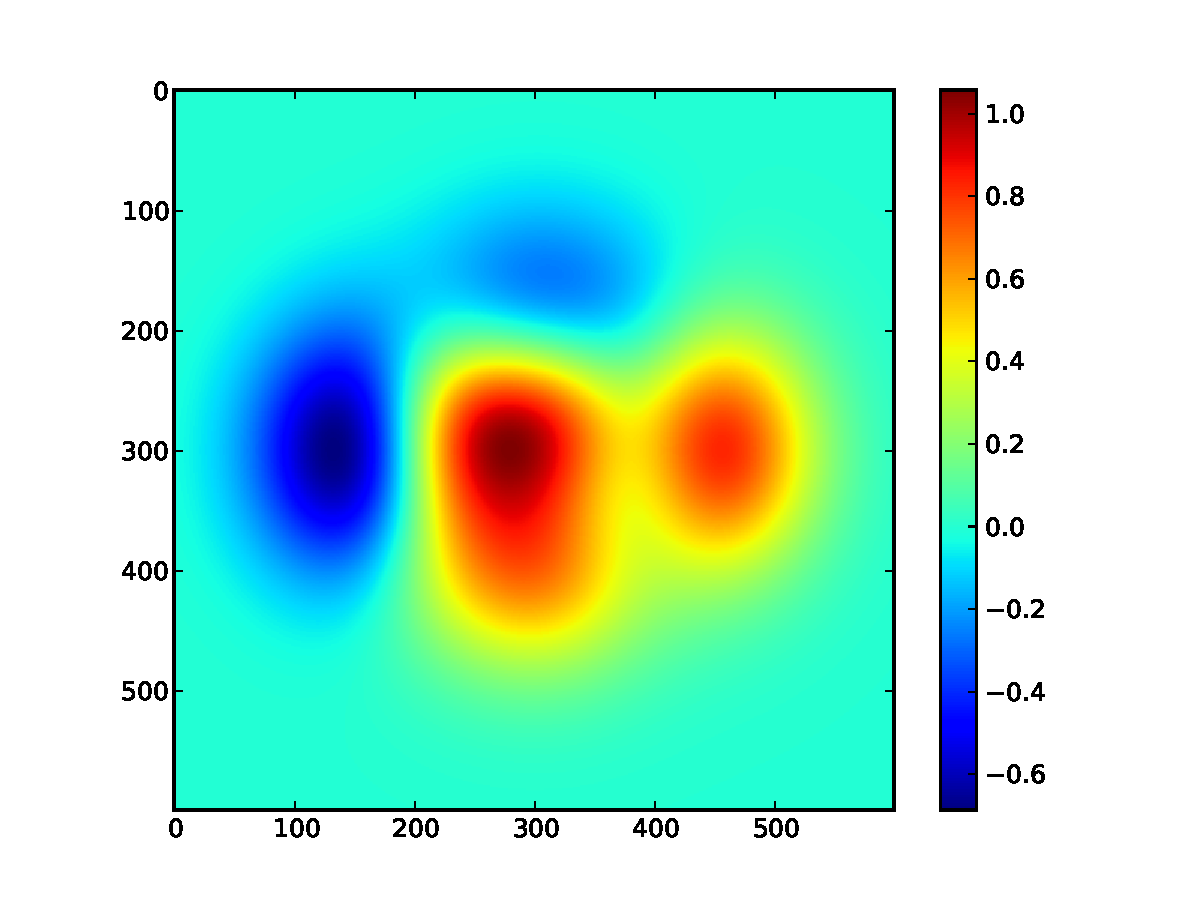
\includegraphics[width=0.6\textwidth]{Chapter-2/figs/color}
  \caption{A figure at the top of the page.}
  \label{fig:ch3.1}
\end{figure}
%
\lipsum[2]
%
\begin{figure}[!h]
  \centering
  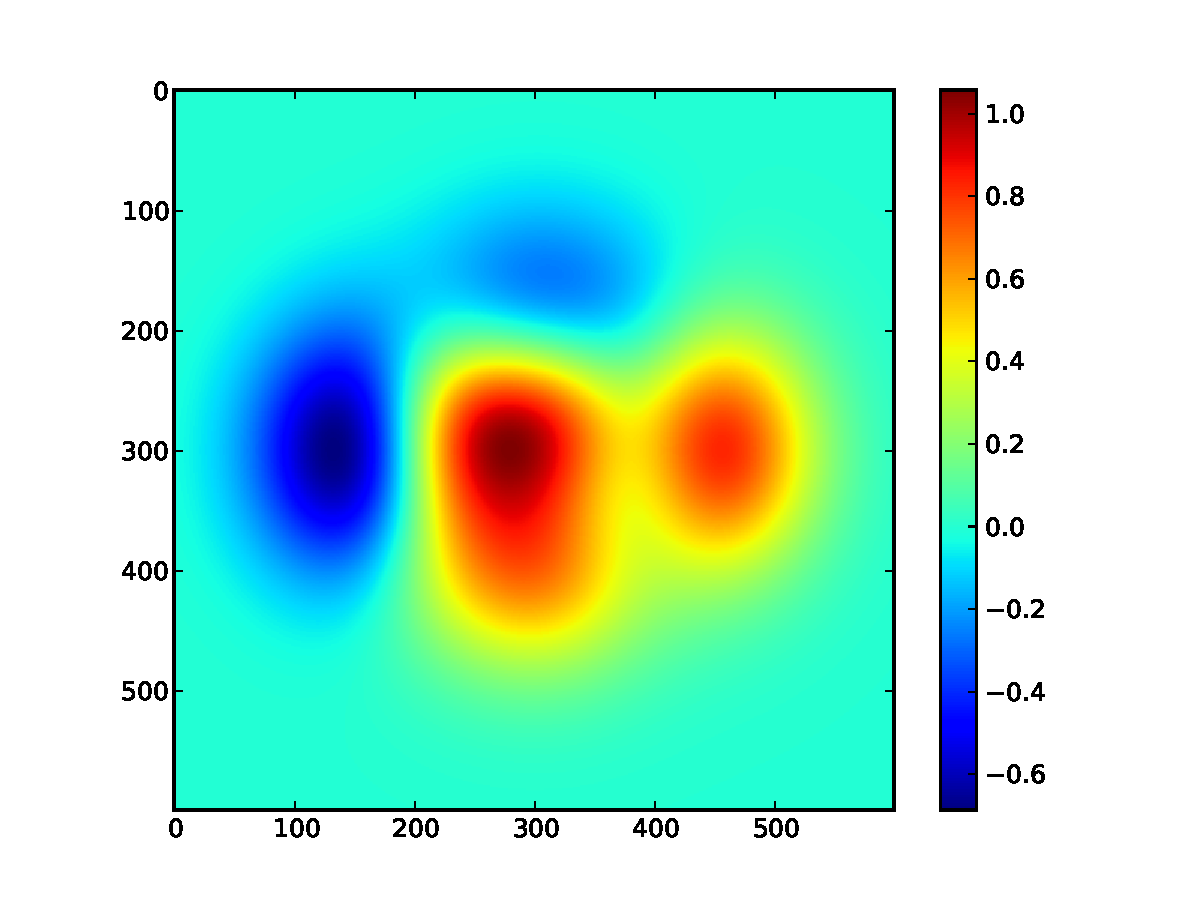
\includegraphics[width=0.6\textwidth]{Chapter-2/figs/color}
  \caption{A figure in the middle of text.}
  \label{fig:ch3.2}
\end{figure}
%
\begin{figure}[!b]
  \centering
  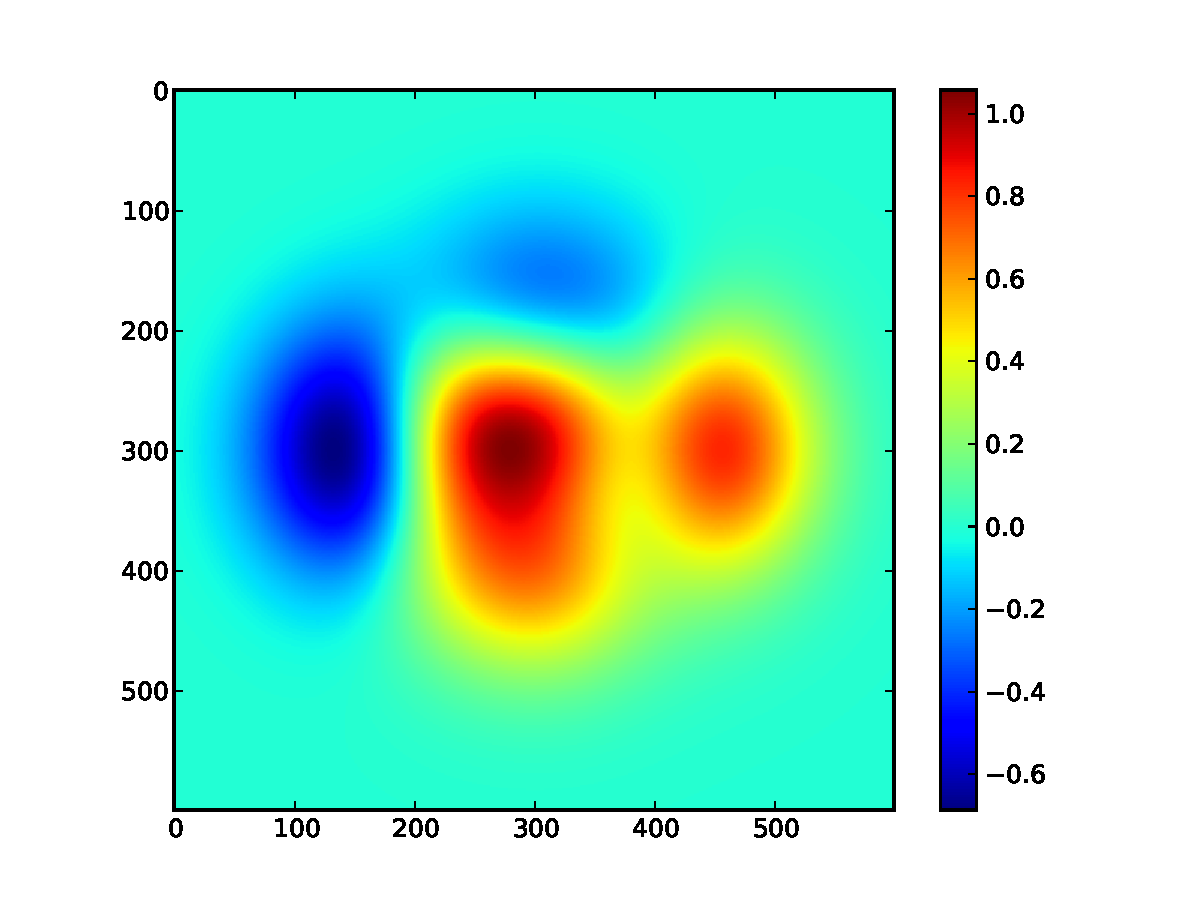
\includegraphics[width=0.6\textwidth]{Chapter-2/figs/color}
  \caption{A figure at the bottom of the page.}
  \label{fig:ch3.3}
\end{figure}
%
\lipsum[3]

%\chapter{Methodology}

\section{Corrosion}

One of the main phenomenon that affect the long term behavior of RC structures is corrosion of the reinforcing steel. Two types of corrosion are possible:
\begin{itemize}
		\item Carbonation, 
		\item Chloride attack
\end{itemize}

The main source of corrosion in most RC structures is Chloride Attack and is the one that is assumed in the present study.

Corrosion of steel in concrete is an electrochemical process \cite{Mehta2014} this corrosion mat be generated in two ways:
\begin{itemize}
	\item Composition cells may be formed when to dissimilar metals are embedded in concrete or when significant variations exist in the surface characteristics of steel
	\item In the vicinity of steel concentration cells may be formed due to differences in the concentration of dissolved ions, such as alkalies and \textbf{chlorides}.
\end{itemize}

The corrosion process under chloride attack type of corrosion consists in first the protective film  on the reinforcing steel surface is destroyed, a process known as \textbf{depassivation}, then initiation of corrosion happens, the electrical resistivity and the oxygen content control corrosion. Figure \ref{fig:corr1} schematically show this process.

\begin{figure}[htbp]
\centering
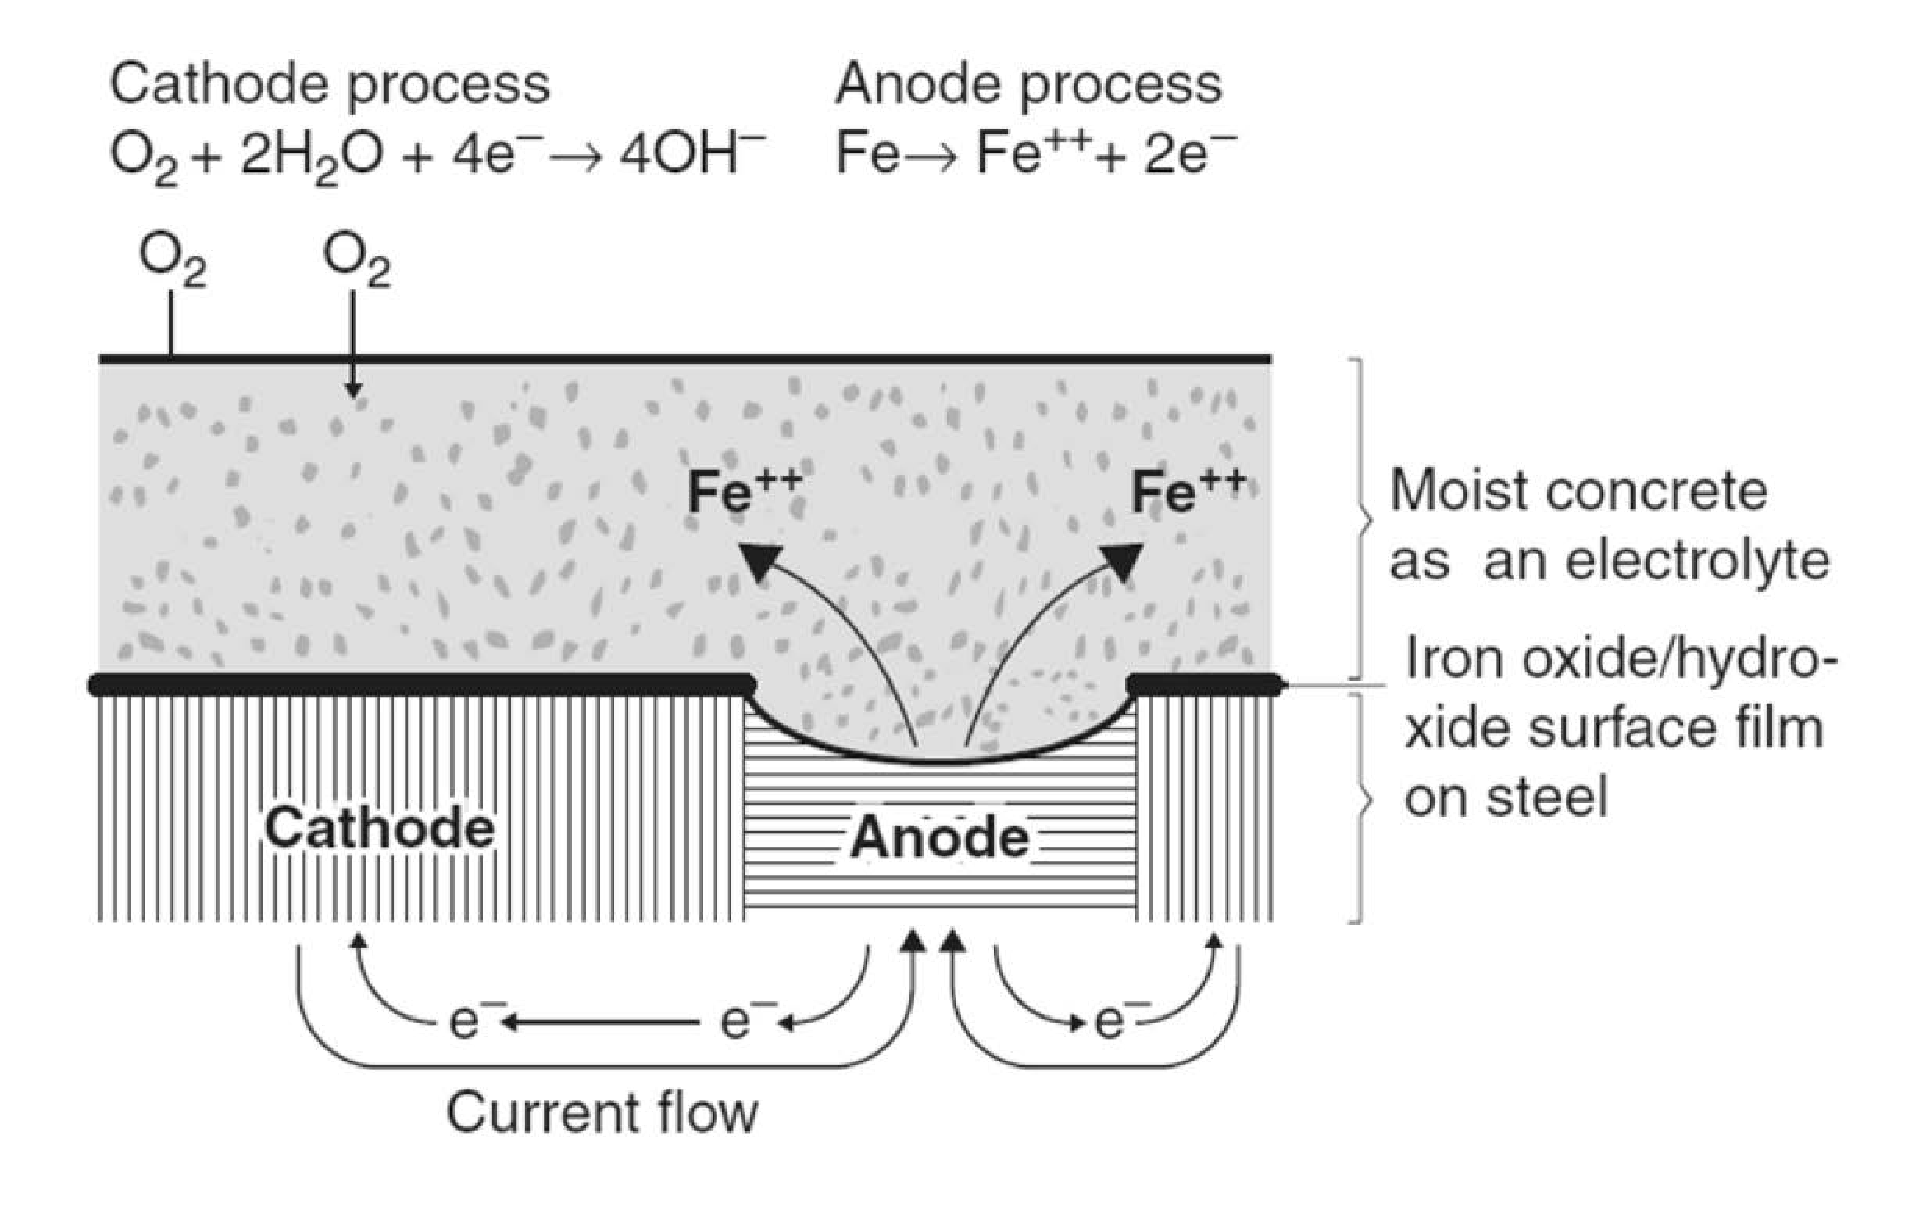
\includegraphics[width=0.9\textwidth]{Chapter-2/figs/Corrosion_Process}
\caption{Corrosion Process in Reinforcing Steel Bar \cite{Mehta2014}}
\label{fig:corr1}
\end{figure}


A literature review to characterize corrosion in reinforcing steel is presented such that corrosion can be modeled as a function of time, the corrosion process is an extensive field of research and to characterize it, therefore the different components of this subject are categorized as follows:

\begin{enumerate}
	\item Time to Initiation of Corrosion (Tcorr)
	\item Corrosion growth in reinforcing steel
	\item Mechanical Properties of Corroded Reinforcing Steel (fycorr, fucorr)
	\item Cyclic Test on Corroded RC Columns
	\item Flowchart of Corrosion Model Implemented
\end{enumerate}

 
\subsection{Time to Corrosion}

Time to corrosion refers to the corrosion initiation at which the passivation of steel is destroyed and reinforcement starts corroding actively.
\newline

\textbf{Christensen Model}
\newline

Christensen \cite{Thoft-Christensen} main goal was to generate a corrosion model that was general for all concrete elements, additionally the authors tried to generate a model that also included the appearance of cracks due to corrosion that would evetually grow and the spall the concrete. 

More specifically related to reinforcing steel corrosion they developed a model based on Fick's law of diffusion to model the rate of chloride penetration into concrete as a function of concrete cover and time. 

\begin{equation}
	\frac{\partial C(x,t)}{\partial t} = D_c \frac{\partial C(x,t)}{\partial x^2}
	\label{eq:one}
\end{equation}

After solving equation \ref{eq:one} the following expression results:
\begin{equation}
  T_{corr}=\frac{d^2}{4D_c} \left[erf^{-1}\left(\frac{C_{cr}-C_{0}}{C_1 -C_0}\right)\right]
  \label{eq:two}
\end{equation} 

$d$: Concrete cover

$D_0$: Diffusion coefficient

$C_{0}$: Equilibrium Chloride Concentration

$C_{cr}$: Critical chloride corrosion concentration
\newline

While this model provides a means to calculate the Time for initiation of corrosion as a function of Concrete Cover and Diffusion concentration, the estimation of the Diffusion concentration depends on several factors such as environment, curing and water to cement ratio it is not a reliable method to estimate the Time to Corrosion.
\newline

\textbf{Gosh \& Padgett Model}
\newline

Ghosh et al calculate time to corrosion based on Thoft-Christensen model, considering in-field corrosion related studies of existing bridge components in the United States exposed to deicing salts to obtain mean values of chlorides concentration and put them in a modified version of the Thoft-Christensen Model.

\begin{equation}
T_{corr}=\frac{x^2}{4 D_c} \left[erf^{-1} \left(\frac{C_0-C_cr}{C_0} \right) \right]^{-2}
  \label{eq.three}
\end{equation} 

$D_c$ 1.29 $frac{cm^2}{year}$ Diffusion Coefficient 

$C_0$ 0.10 Surface Chloride Concentration

$C_r$ 0.04 Critical Chloride Concentration
\newline

While this model provides mean values for the time of initiation of corrosion, it is limited to environments that are controlled by \textbf{dicing salts only}.
\newline

\textbf{Life 365}
\newline

Is a software developed by a consortium of companies of the cementitious materials industries and academic institutions. This software relies on the studies summarized above, mainly using the Thoft-Christensen model, but as opposed to assuming dicing environments only, this software uses a database of chlorides concentration for different location in the USA and Canada, which gives more accurate results depending on the location and environment in which the structure is located.

While this is a more robust model to obtain the initiation of corrosion since it considers the location and environment of the structure and it also has the ability to include other durability issues, it is difficult to implement in a batch run format since the program is in a closed format.
\newline

\textbf{Liu \& Weyers Model}
\newline

\begin{equation}
  T_{cr}=\frac{W_{crit}^2}{2k_p}
  \label{eq.four}
\end{equation} 

\begin{equation}
  W_{crit}=\rho_{rust} \left[ \pi \left[ \frac{C f'_t}{E_{ef}} \left( \frac{a^2+b^2}{a^2-b^2}+\nu_c \right)+d_o \right] D+ \frac{W_{st}}{\rho_{st}} \right]
  \label{eq.five}
\end{equation} 

\begin{equation}
  k_p=0.098 (\frac{1}{\alpha})\pi Di_{corr}
  \label{eq.six}
\end{equation} 

$W_{crit}$: Critical amount of corrosion needed to induce cracking.

$W_{st}$: Mass of corroded steel.

$\rho_{rust}$: Density of rust material.

$\rho_{st}$: Density of steel.

$f'_t$: Tensile strength of the concrete. 

$E_{ef}$: Effective elastic modulus of concrete $E_{ef}=\frac{E_c}{1+\phi_{crit}}$ 

$\phi_{crit}$ Creep coefficient of the concrete.

$D$: Diameter of bar.

$d_o$: Thickness of pore band around the steel/concrete interface.

$\nu_c$: Poisson's ratio of concrete.

$C$: Cover depth

$a=\frac{D+2d_o}{2}$

$b=C+\frac{D+2d_o}{2}$

\subsection{Rate of corrosion}

\textbf{Vu et al. Model }
\newline

To estimate the loss of steel cross section due to corrosion a time dependent corrosion rate model was developed by \cite{Vu2000}, this model implies that corrosion diminishes with time since as corrosion accumulates with time around the steel, it precludes uncorroded steel to react with the environment. The model is shown in \eref{eq.five}.

\begin{equation}
  i_{corr}=\frac{37.5(1-w/c)}{d_c}
  \label{eq.eight}
\end{equation} 

$w/c$: Water Cement ratio
$d_c$: Cover depth

In \fref{fig:hist1} the behavior of this model for different values of $w/c$ ratios is shown. It can be seen that at larger values of cover depth the rate of corrosion decreases rapidly and as the water cement ratio increases the rate of corrosion decreases.
%
\begin{figure}[htbp]
\centering
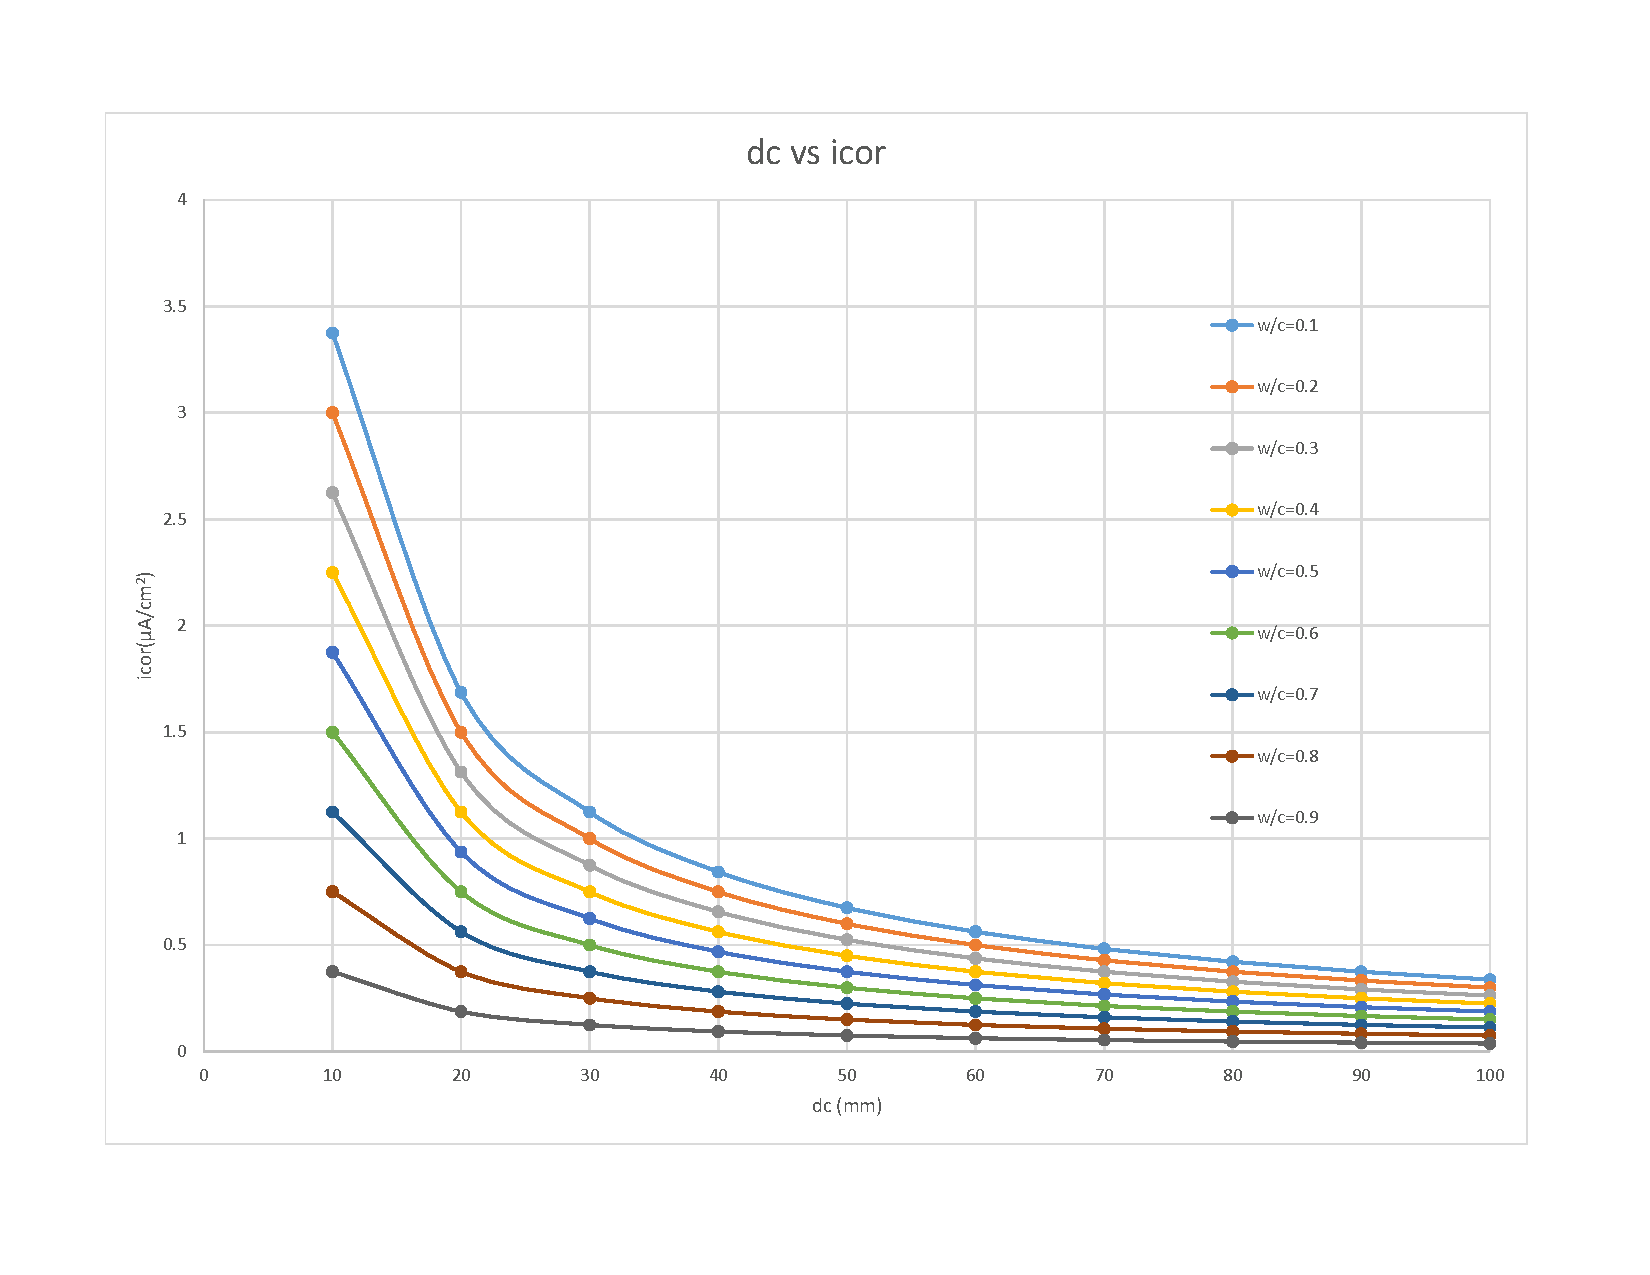
\includegraphics[width=0.7\textwidth]{Chapter-1/figs/dcvsicor}
\caption{Concrete cover depth vs rate of corrosion}
\label{fig:hist1}
\end{figure}

From the Vu et al model the diamater degradation is calculated according to Choe et al as:

\begin{equation}
  d_{corr}=d_{bi}-\frac{1.0508(1-w/c)}{d_c} (t-t_{corr})^{0.71}
  \label{eq.nine}
\end{equation} 

$d_{bi}$: Is the initial diameter of the bar

The diameter is plotted in \fref{fig:hist2}.

\begin{figure}[htbp]
\centering
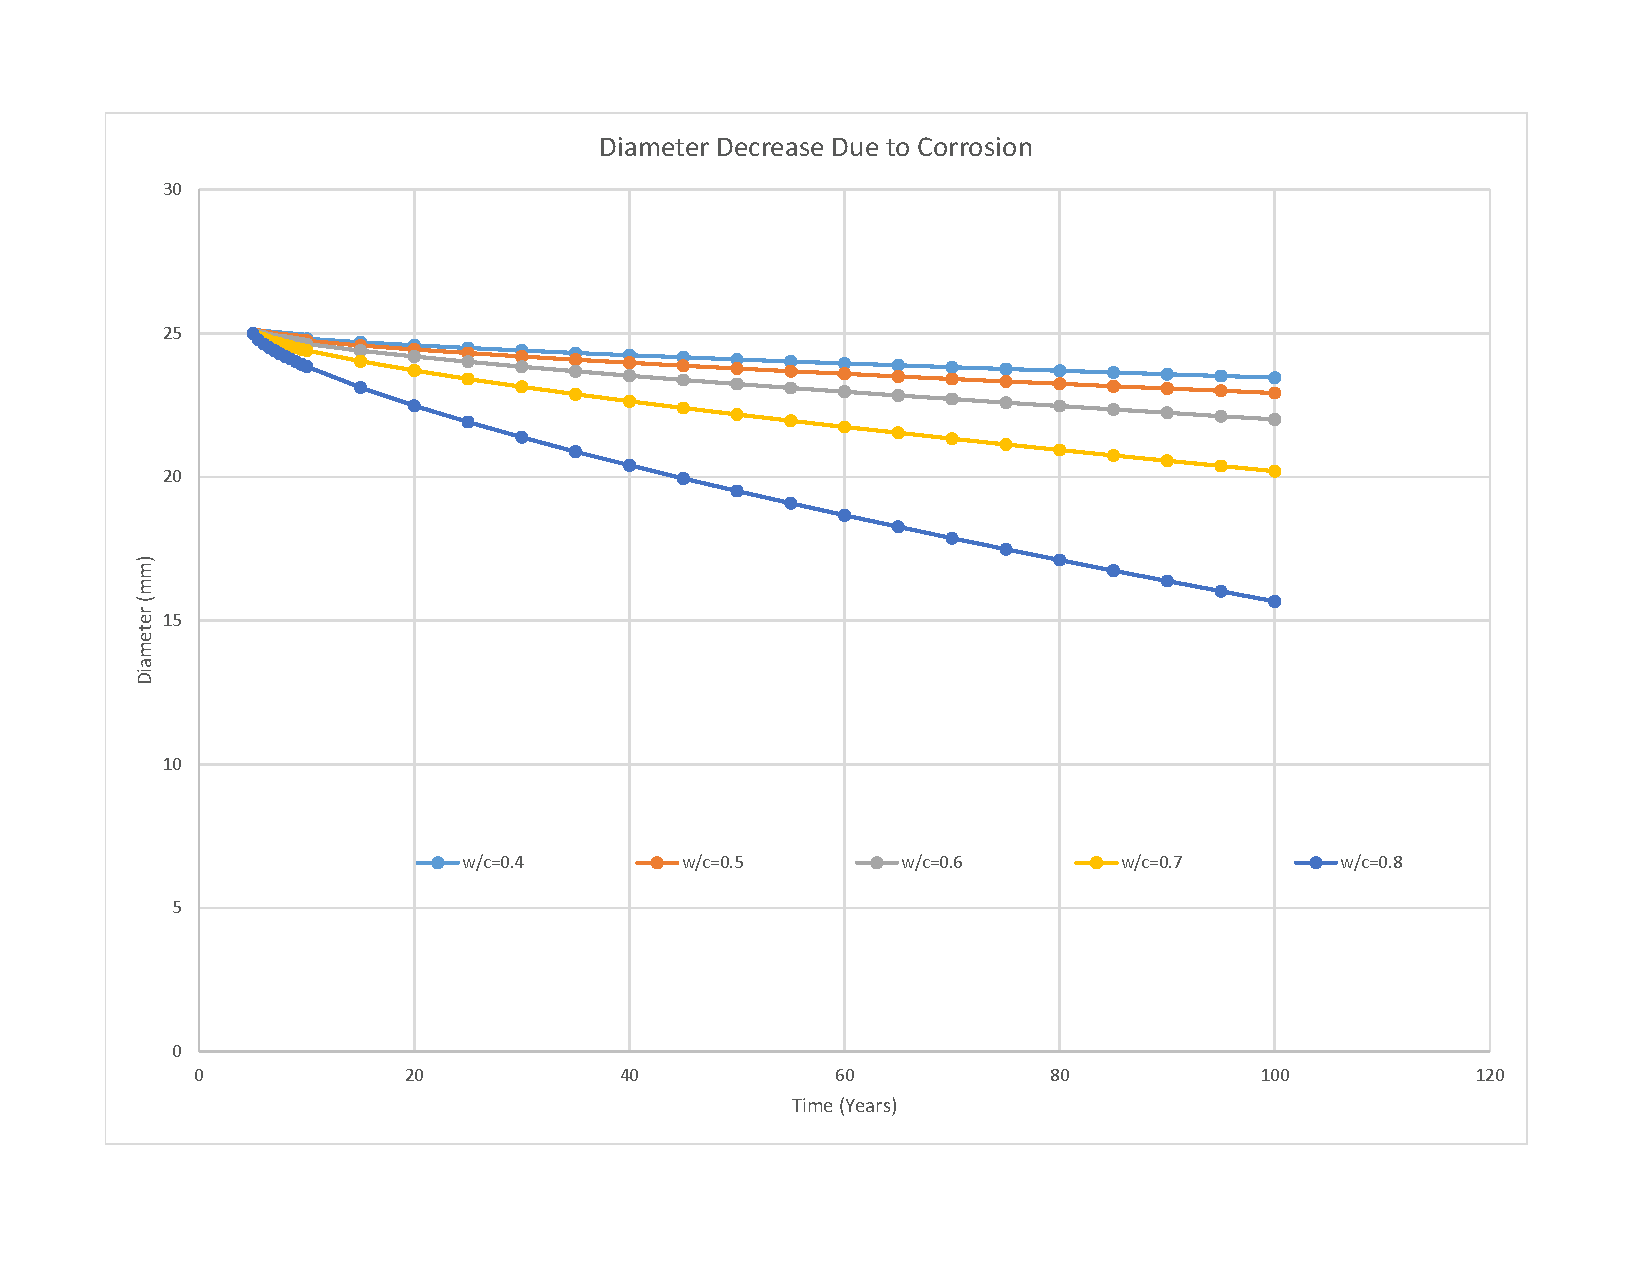
\includegraphics[width=0.7\textwidth]{Chapter-1/figs/DiameterDecrease}
\caption{Diameter decrease due to corrosion}
\label{fig:hist2}
\end{figure}

These values would correspond to a level of corrosion that varies from 7\% corrosion to 21\% of corrosion for w/c ratios that ranges from 0.4 to 0.6
The level of corrosion is calculated as:

\begin{equation}
  C=\frac{G_o-G}{g_ol_o} *100%
  \label{eq.ten}
\end{equation} 

Then the Corrosion level is plotted as a function of time in \fref{fig:hist3}

\begin{figure}[htbp]
\centering
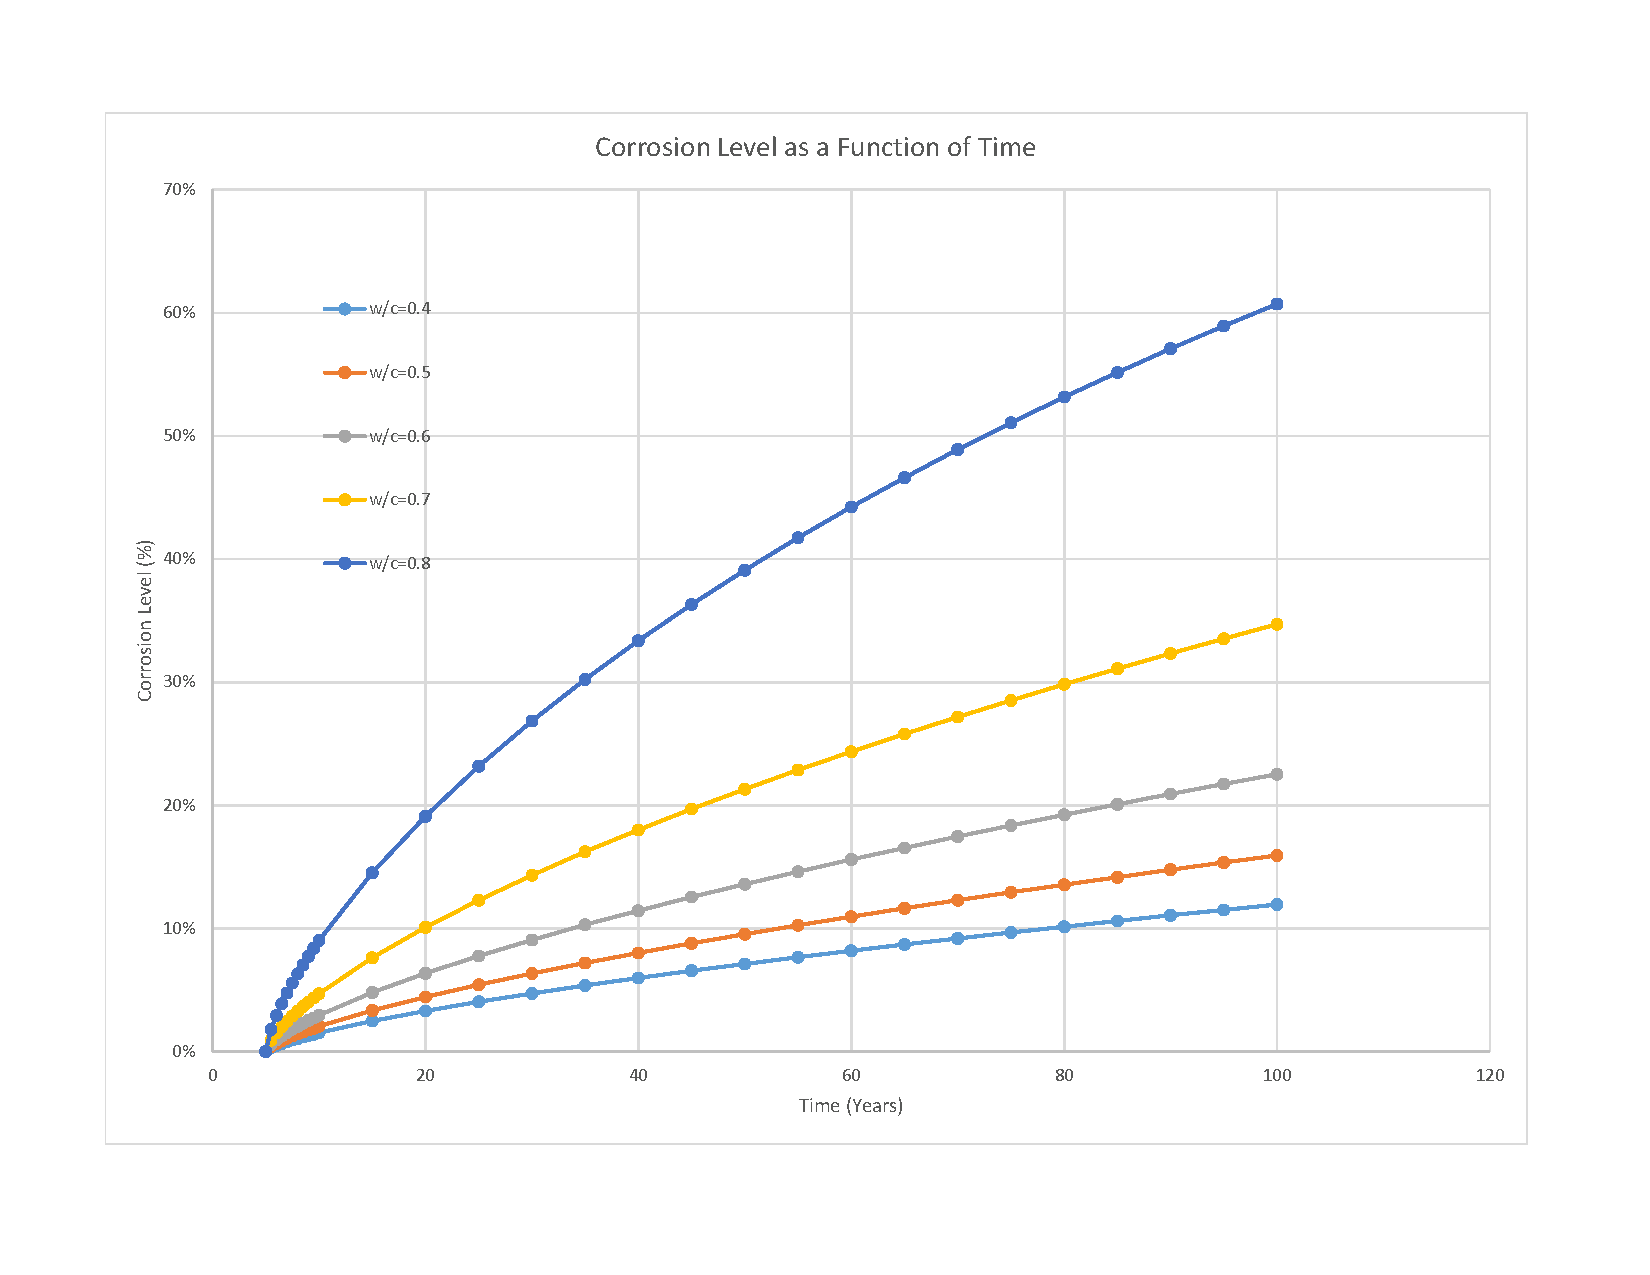
\includegraphics[width=0.7\textwidth]{Chapter-1/figs/CorrosionLevel}
\caption{Corrosion Level vs Time (years)}
\label{fig:hist3}
\end{figure}

\subsection{Corrosion modified properties of reinforcing steel bars}

In a study presented by Yuan et al \cite{Yuan2017a} it was shown from experimental results that the mechanical properties of steel for different levels of corrosion could be modified for analysis as follows:

\begin{equation}
  f_{y,C}=f_{yo}(1-0.021C)
  \label{eq.eleven}
\end{equation} 

\[
  f_{u,C}=f_{yo}(1.018-0.019C)
\]
\[
  \delta_{s,C}=\delta_{so}(1-0.021C)
\]
\[
  \varepsilon_{y,C}=\varepsilon_{yo}(1-0.021C)
\]

\:
\textbf{Choe et al. Model }
\:
Choe et al research is a seismic fragility estimates for RC columns subjected to corrosion, while the study is probabilistic in nature it defines the reduction in rebar cross section as:

\begin{equation}
	d_{b}(t)=d_{bi}-2\int_{T_{corr}}^{t} \lambda(t) dt
\end{equation}

Considering the model proposed by Vu et al the bar diameter degradation can be expressed as:

\begin{equation}
	d_{b}(t)=d_{bi}-\frac{1.508(1-\frac{w}{c})^-1.64}{d}(t-T_{corr})^0.71
\end{equation}

Where the diameter of the bar and the cover is in (mm).
Pros:
Easy way to calculate the reduction of bar diameter.
Cons:
The model carries out the assumptions made by Vu et al. concerning concentration of chlorides assumed and the diffusion assumed.

With this information, the corrosion level is calculated as:

\begin{equation}
	CL=\frac{d_{i}-d(t)}{d_{i}}
\end{equation}

\subsection{Corrosion modified properties of reinforcing steel bars}
\:
\textbf{Yuan et al. 2017}
\:
Yuan et al performed full-scale tests on columns with corroded longitudinal reinforcement, with which they proposed the following equation to characterize the effects of corrosion in reinforcing steel.

\begin{equation}
	f_{y}(t)=f_{y0}(1+0.021CL)
\end{equation}

While the equation showed, agreement with the test results that they performed it has not been corroborated by other researchers. In the current consensus, the model used is the one proposed by Du et al.


\textbf{Du et al. 2005}

Du et al investigated the effect of corrosion on the mechanical properties of steel using corrosion levels of 5%, 10%, 15% and 20%. Another variable that was researched was the type of rebar (smooth or ribbed), diameter of the rebar.
\begin{equation}
	f_{y}(t)=f_{y0}(1+0.021CL)
\end{equation}

\section{Steel Strain Aging}

\subsection{Metallurgical Process}

It is generally accepted that strain aging is due to the diffusion of carbon and/or nitrogen atoms in solution to dislocations that have been generated by plastic deformation. Initially, an atmosphere of carbon and nitrogen atoms is formed along the length of a dislocation, immobilizing it. Extended aging, however, results in sufficient carbon and nitrogen atoms for precipitates to form along the length of the dislocation.

These precipitates impede the motion of subsequent dislocations, and result in some hardening and loss in ductility. The extent of strain aging, which is a thermally activated process, depends primarily on aging time and temperature. In general, extended aging results in a saturation value above which further aging has no effect.

A second strengthening mechanism occurs when cold deformation (alone) is applied to steels. When dislocations break away for their pinning interstitial atoms and begin the movement causing slip they begin to intersect with each other. A complex series of interactions between the dislocations occurs, causing them to pin each other, decreasing their mobility. The decreased mobility also results in higher strength, lower ductility and lower toughness. As a result, cold deformed steels already have lowered ductility and toughness before any strain aging occurs and when heating follows cold deformation, the loss in ductility and toughness is greater. It is this combination of events that is the most damaging to the toughness of structural steels.

\subsection{Strain aging effects in structures}

Since it has already been established that strain aging is the process in which steel after being subjected to large strains develops an increased strength and reduced ductility with time and therefore important to include it in a time dependent analysis, considering the fact that plastic hinges will form in a ductile structure and the steel could reach high strains in this regions of the structure. Furthermore strain aging will cause an increased in the strength of the plastic hinge and as a consequence plastic hinges might be formed in regions of the structures that have not been designed for such demands. The effects of strain aging may also alter the transverse reinforcement due to both cold bending, making them susceptible to brittle failure.

According to \cite{Restrepo-Posada1994} most strain aging occurs in the first 37 days. Also \cite{Momtahan2009} studied strain aging effects with respect to time for different levels of pre-strains that ranged from $2\varepsilon_y - 10\varepsilon_y$ and for a time frame of 3 days to 50 days, from this study it was determined that a significant effect of strain aging took place from pre-strains $5\varepsilon_y$ and on. Strains higher than $15\varepsilon_y$ indicate a performance level in which substantial damage has been induced in the structure such that it is deemed unrepairable and therefore pre-strains higher that $15\varepsilon_y$ are unpractical and not studied by Montahan et al\cite{Momtahan2009}.
\\
\textbf{Momtahan et al Strain Aging Effects in Yield Strength of Steel}

Momtahan et al was able to correlate the increase in yield strength as a function of time and the pre-strain in reinforcing steel bars. The proposed equations are shown below:

\begin{figure}[htbp]
\centering
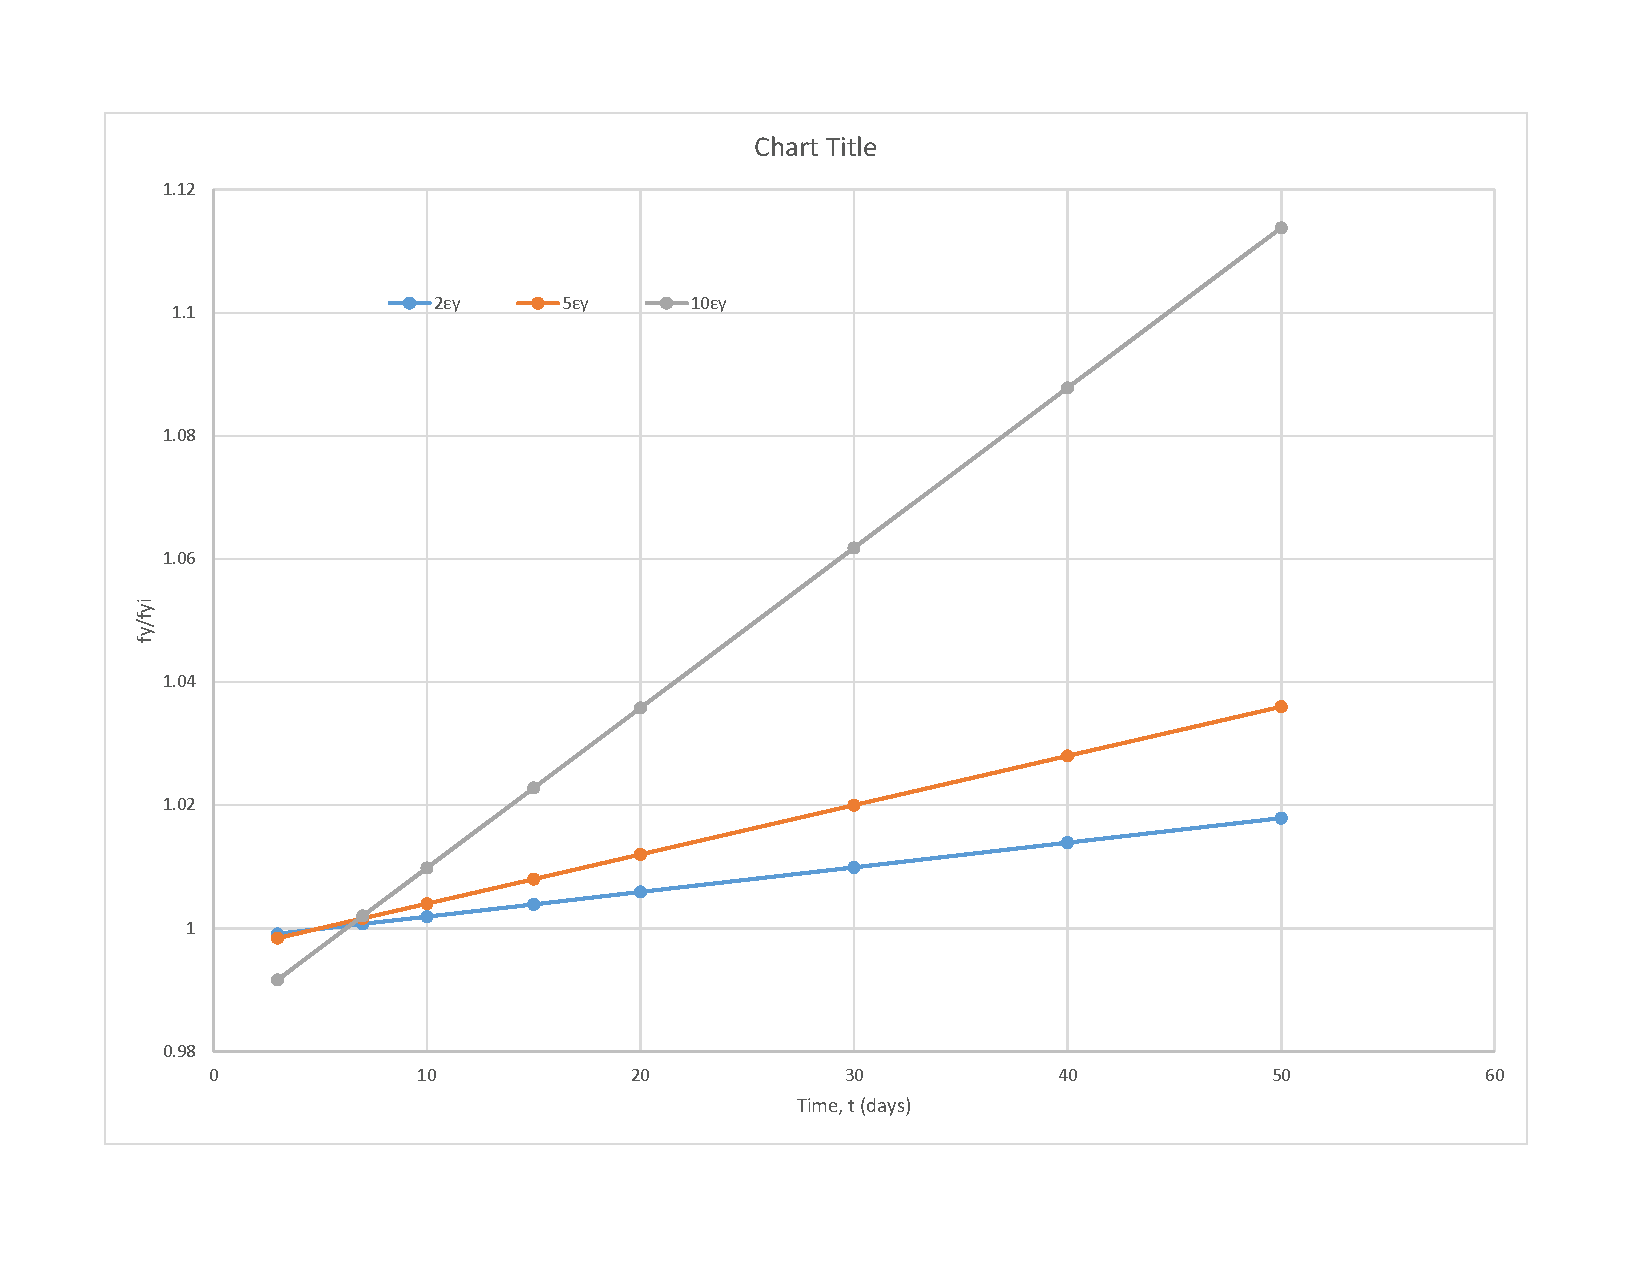
\includegraphics[width=0.9\textwidth]{Chapter-1/figs/StrainAging_TimeDependent}
\caption{Strain Aging effect on Yield Strength vs Time (days)}
\label{fig:hist4}
\end{figure}


For $10\varepsilon_y$

\begin{equation}
  \frac{f_y}{f_{yi}}=0.0026t+0.9838
  \label{eq.twelve}
\end{equation} 

For $5\varepsilon_y$

\begin{equation}
  \frac{f_y}{f_{yi}}=0.0008t+0.996
  \label{eq.thirteen}
\end{equation} 

For $2\varepsilon_y$

\begin{equation}
  \frac{f_y}{f_{yi}}=0.0004t+0.9979
  \label{eq.fourteen}
\end{equation} 

It is proposed to limit the increase in yield strength to the one obtained at 50 days. These equations are plotted in \fref{fig:hist4}

\section{Experimental campaign}

\section{Multiple Seismic Events}

\subsection{Main Shock Series}

\subsection{Main Shock - After Shock Series}

\section{Future Topics}

\begin{itemize}
	\item Concrete Strength Aging
	\item Welding and Fatigue in Steel Structures
	\item Repair Effects
	\item Main Shock - After Shock Series - Repair Series
\end{itemize}

%\chapter{Analytical Model and Preliminary Results}
In this chapter first a framework for the analysis that is performed is presented, later the basic model that is used for the analysis is presented and later calibrated and verified with experimental data available in the literature. Finally preliminary results are presented that will define the general view for the proposed research

\section{Analytical Model}

\subsection{Cantilever Column}
This study focuses on the behavior of a Single Degree of Freedom System representing a Cantilever Reinforced Concrete Column. The column is modeled as shown in \fref{fig:Structural_Model} This structure is modeled in OpenSeesPy \cite{McKenna2010}\cite{Zhu2018} using the $forceBeamColumn$ element \cite{Scott}. The forceBeamColumn element is used with two-point Gauss-Radau integration applied in the hinge regions and two-point Gauss integration applied on the element interior for a total of six integration points \cite{Scott}. The force based formulation requires only a single element to accurately represent the full nonlinear deformation of the member and the integration scheme selected prevents the loss of objectivity during softening response while also providing integration points at the member ends \cite{Calabrese2010},\cite{Scott}. The element requires the length of plasticity be defined at each end of the member, for which the tension based rectangular plastic hinge length is calculated using the following expressions \cite{Goodnight2013}:

\begin{equation}
    L_{pc}=k*L_{eff} + 0.4D
    \label{eq:LP_Comp}
\end{equation}
\begin{equation}
	k=0.2*(Fu/Fy - 1) \leqslant 0.08
	\label{eq:K_Lp}
\end{equation}
\begin{equation}
    L_{pt}=L_{pc}+\gamma*D
    \label{eq:LP_Tension}
\end{equation}

For Single Bending
\begin{equation}
    \gamma=0.33
    \label{eq:Gamma_LPt}
\end{equation}

The two-point Gauss-Radau integration is applied such that each end node integration is weighted equal to the specified plastic hinge length, as illustrated in \fref{fig:Fiber_PlasticHinge}. Therefore, strains recorded at the end sections represent accurate values even in the case where deformation localizes to the ends from strain softening behavior. For the case of the cantilever column considered, only one plastic hinge length is defined, and the opposite end is given an arbitrary unit length. 

\begin{figure}[htbp]
	\centering
	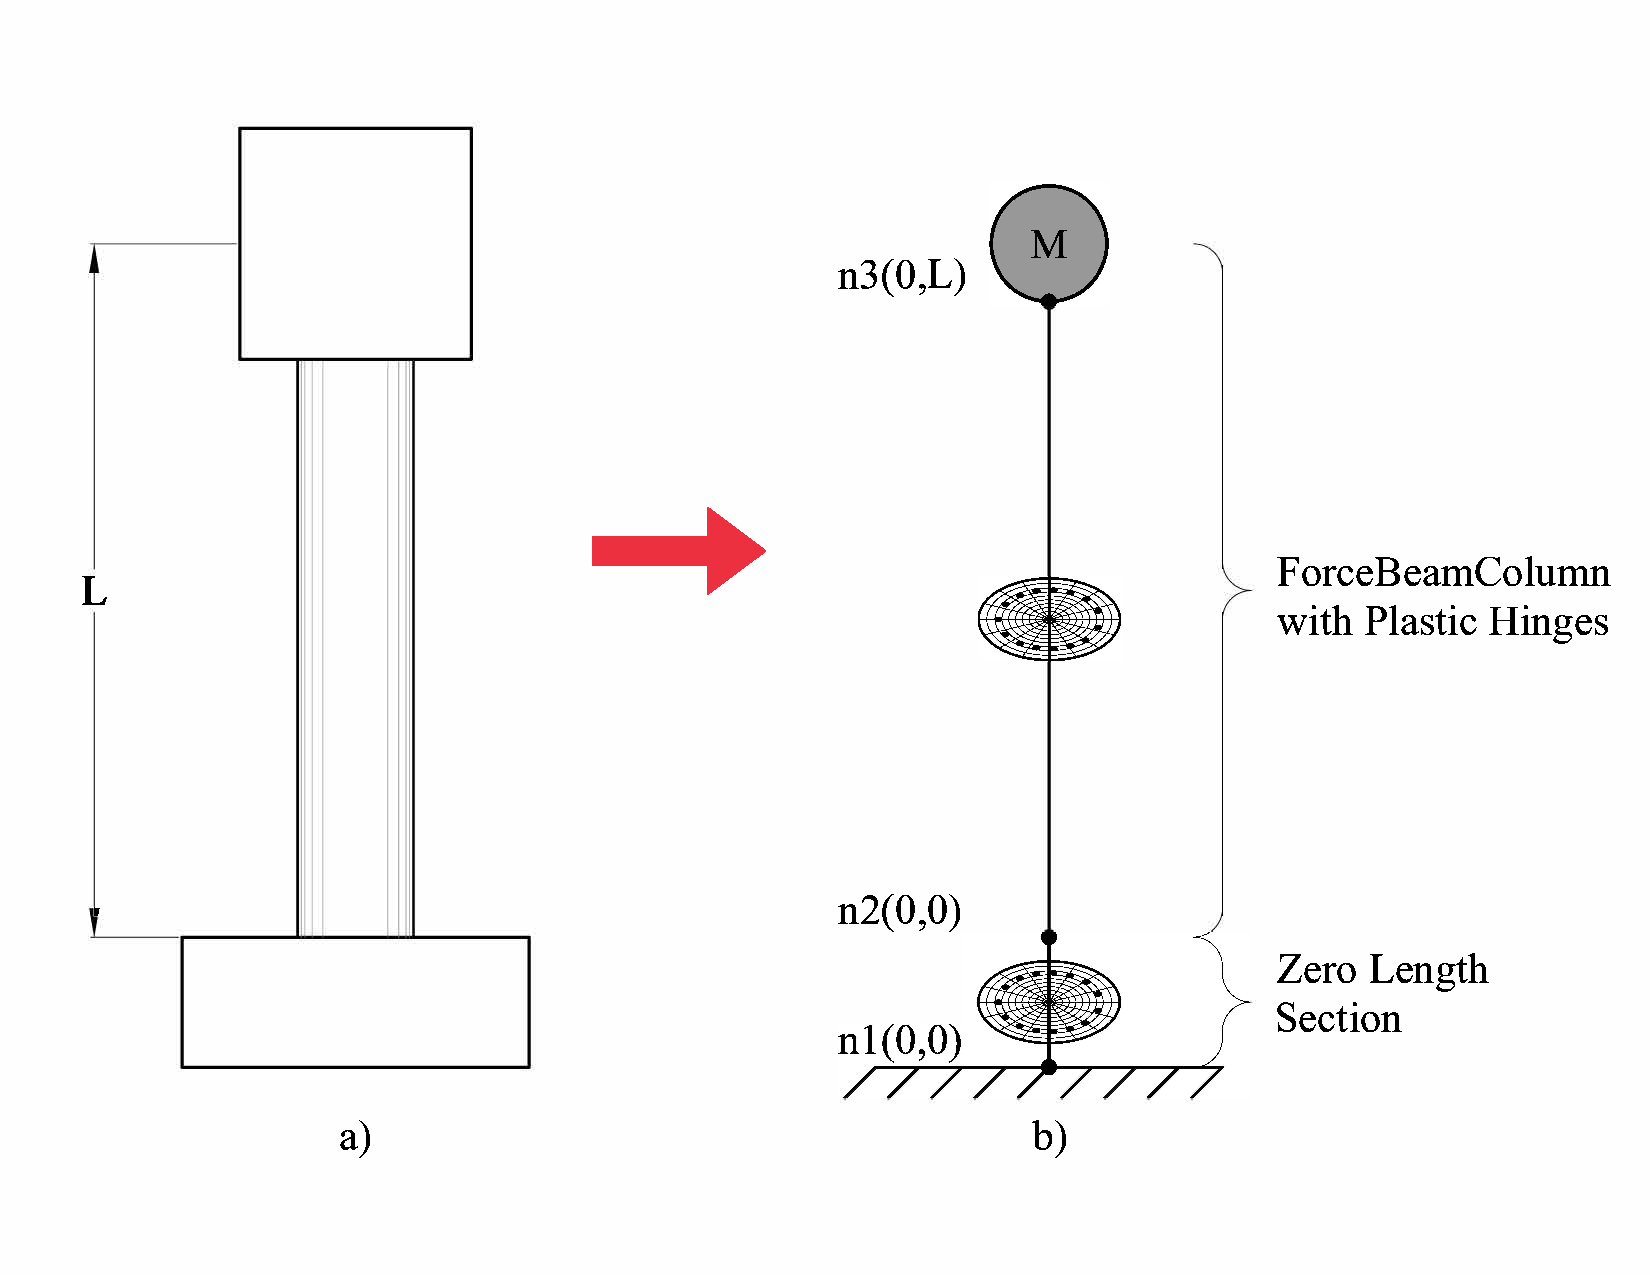
\includegraphics[width=1.0\textwidth]{Chapter-5/figs/StructuralModel_01}
	\caption{Structural Model a) SDOF Column b) Structural Model}
	\label{fig:Structural_Model}
\end{figure}

\begin{figure}[htbp]
	\centering
	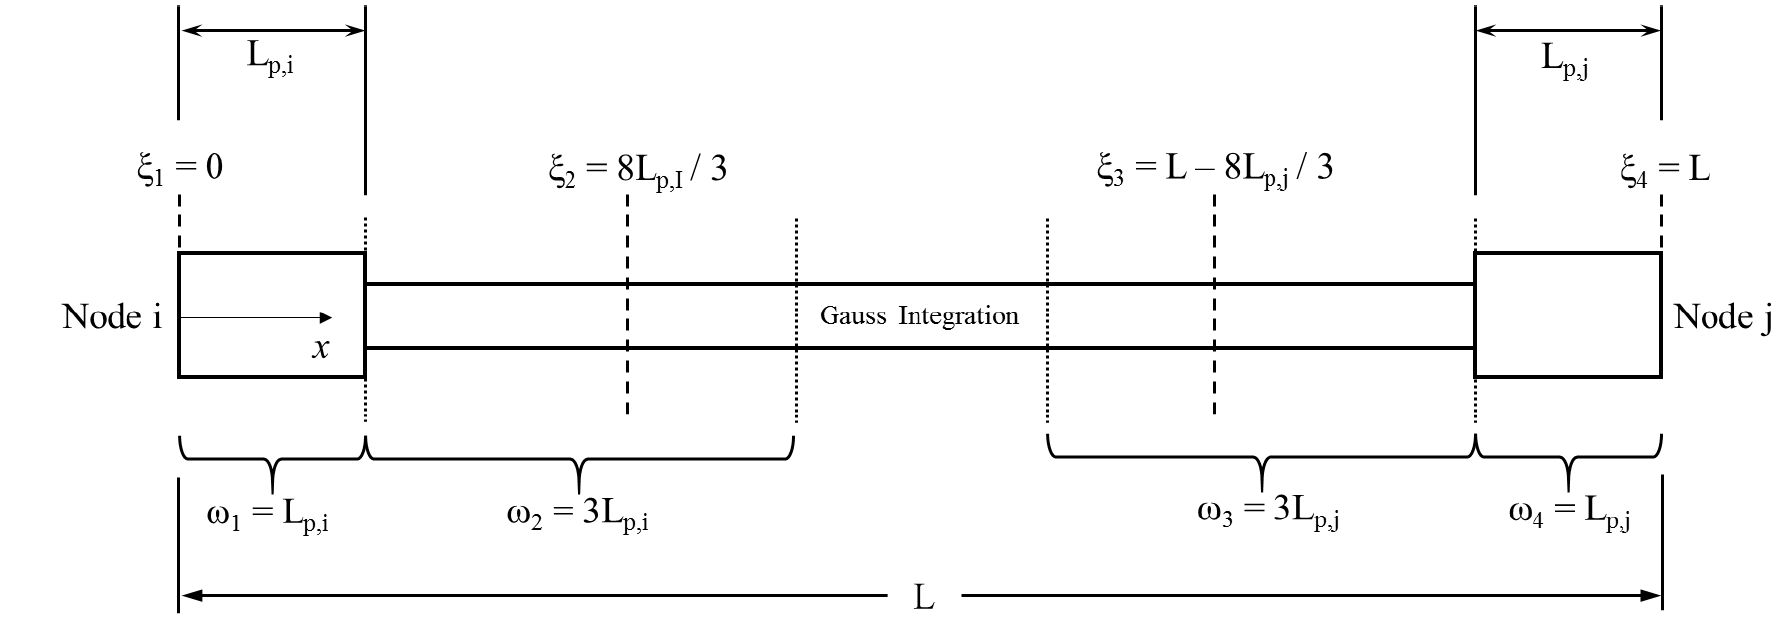
\includegraphics[width=0.9\textwidth]{Chapter-5/figs/fbc_PlasticHinge}
	\caption{End point plastic hinge method \cite{Scott}}
	\label{fig:Fiber_PlasticHinge}
\end{figure}

The section of the column is shown in \fref{fig:ColumnSection}, the section is discretized with concrete and steel material fibers. Concrete fibers are modeled using the $Concrete01$ material, modified for confined material strength based on the Mander confined concrete model \cite{Mander1988}. The $Steel02$ material, based on the Giuffre-Menegotto-Pinto model \cite{Filippou1983} and it is used for the longitudinal reinforcement with recommended parameters ($b = 0.01, R0 = 20, cR1 = 0.925, cR2 = 0.15$). 

\begin{figure}[htbp]
	\centering
	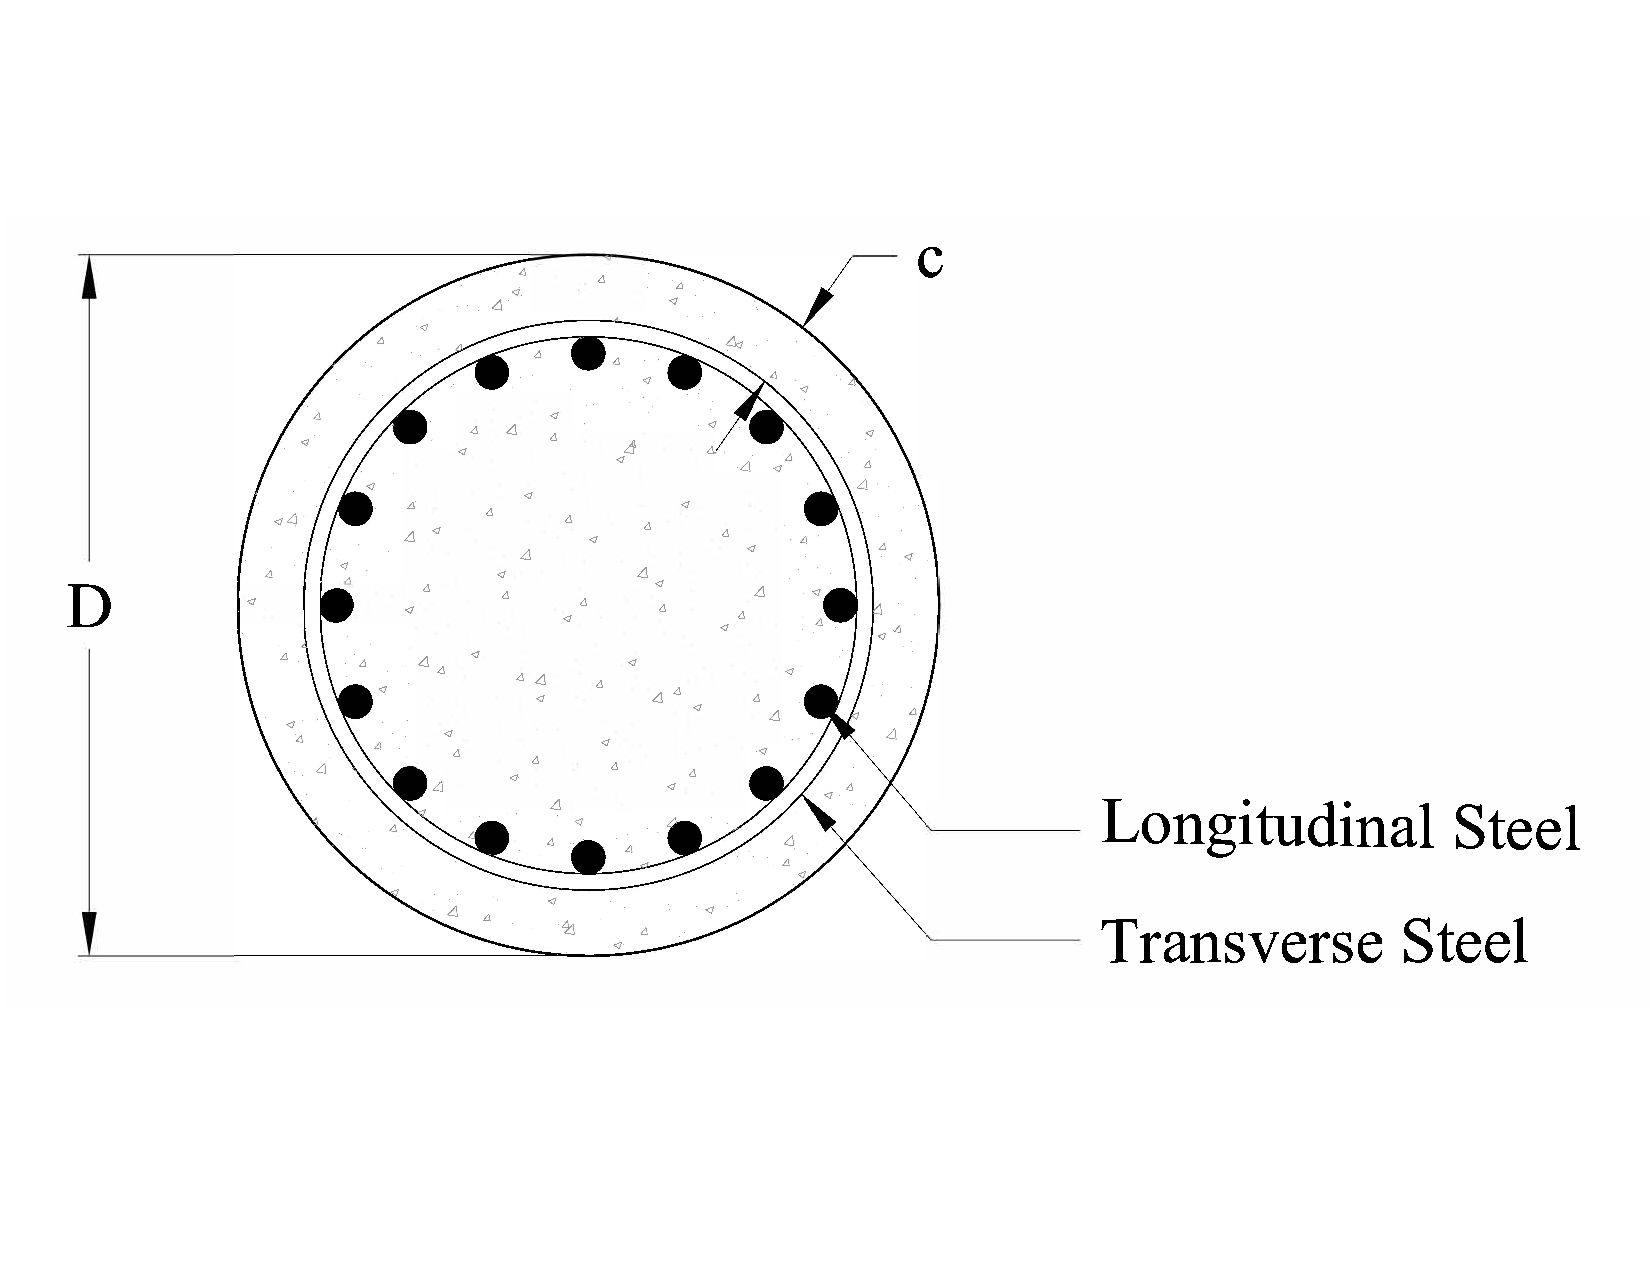
\includegraphics[width=0.7\textwidth]{Chapter-5/figs/StructuralModel_Section}
	\caption{Section of the RC Column}
	\label{fig:ColumnSection}
\end{figure}

\subsection{Strain Penetration Component}

The strain penetration is necessary to be considered to take into account the additional deformation due to anchorage of the reinforcement into the foundation, since the strains of tension in the reinforcement will drop to zero at a depth equal to the true development length of the rebar \cite{Priestley2007}. Experimental studies have generally reported that this end rotation contributes up to 35\% to the lateral deformation of flexural members\cite{Zhao2007} and it is therefore important to incorporate into the analytical model. A way to capture this effect is by using a zero-length section element implemented in nonlinear fiber-based analysis of concrete structures, this is available in the material library of OpenSeesPy as $Bond SP1$ \cite{Zhao2007} this is material model used for the steel fibers of the zero-length section element. 

The required parameters for this model are:
\begin{itemize}
	\item $F_{y}$ Yield strength of the reinforcement steel
	\item $S_{y}$ Rebar slip at member interface under yield stress (see \eref{eq.Rebar_Slip})
	\item $F_{u}$ Ultimate strength of the reinforcement steel
	\item $S_{u}$ Rebar slip at the loaded end at the bar fracture strength a value of $35 S_{y}$ is recommended \cite{Zhao2007}
	\item $b$ Initial hardening ratio in the monotonic slip vs. bar stress response $b=0.45$ is recommended \cite{Zhao2007}
	\item $R$ Pinching factor for the cyclic slip vs. bar response $R=1.01$ is recommended \cite{Zhao2007}
	\item $d_b$ Rebar diameter
	\item $f'c$ Concrete compressive strength of the adjoining connection member
	\item $\alpha$ Parameter used in the local bond-slip relation and can be taken as $\alpha=0.4$ in accordance with CEB-FIP Model Code 90 \cite{CEB1993}
\end{itemize}

Bar slip is calculated as:
\begin{equation}
	S_{y}(in)=0.1\left(\frac{d_{b}F_{y}}{4000\sqrt{f'_{c}}}\left(2\alpha+1\right)\right)^{\frac{1}{\alpha}}+0.013 (in)
	\label{eq.Rebar_Slip}
\end{equation}
\subsection{Design Limit States}
In Performance Based Design (PBD)philosophy different performance levels are defined such that design is controlled such that it is not exceeded for a given demand. 
\section{Comparison with existing physical Tests}
\subsection{Pristine Condition Columns}
\lipsum[2]

\subsection{Accelerated Corrosion Columns}
\lipsum[3]

\section{Analytical Framework}

An overall analytical framework is established such that several analysis can be performed. From this analysis it is possible to determine the effects of damage in the performance of structures. The proposed analytical framework consists in:

\begin{enumerate}
	\item Geometrical Properties of the SDOF column 
	\item Properties of the material are evaluated (i.e. water to cement ratio, cover)
	\item For equal periods of time the Time Dependent Properties are modified
	\item Nonlinear Time History Analysis are performed for discrete events or sequence of events
	\item Results are obtained and evaluated
\end{enumerate}

This procedure has been summarized in the form of a flow chart presented in \fref{fig:NLTHA_Framework}

\begin{figure}[htbp]
	\centering
	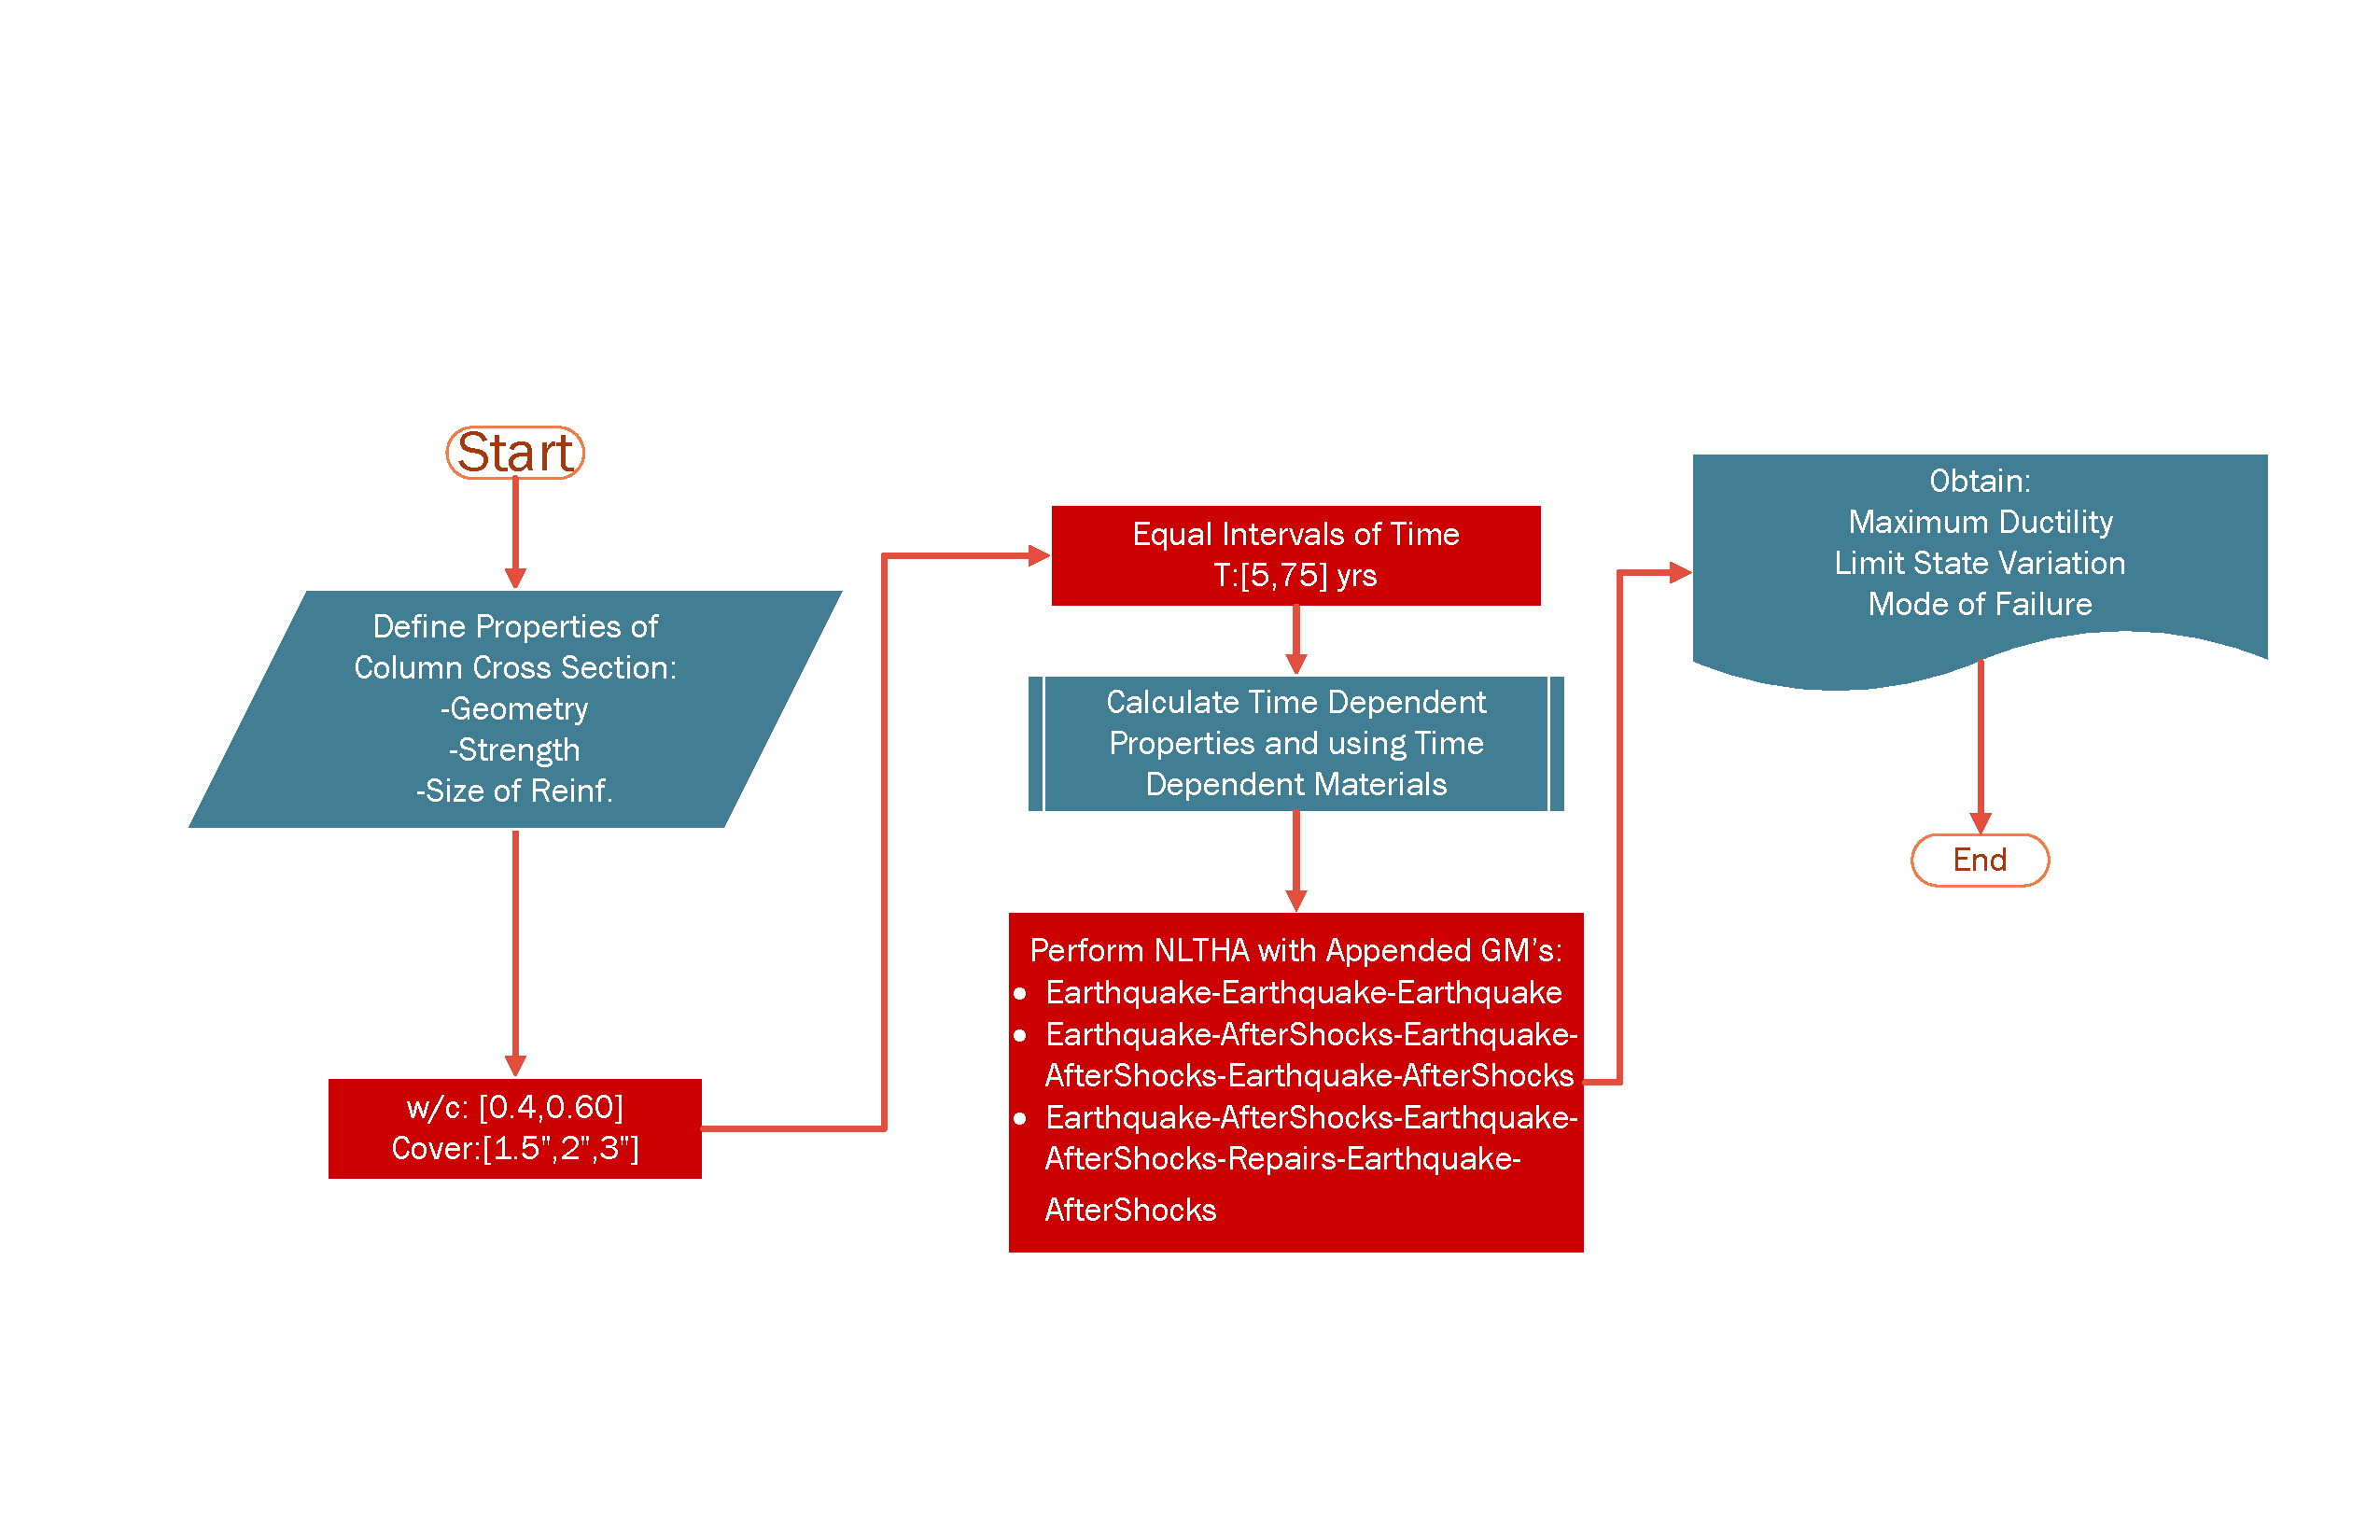
\includegraphics[width=0.9\textwidth]{Chapter-5/figs/AnalysisFramework_01}
	\caption{Analysis Framework Flowchart}
	\label{fig:NLTHA_Framework}
\end{figure}

\section{Earthquake selection}
\lipsum[4]
\section{Results from NLTHA}
\lipsum[5]
\subsection{Effect on global response}
\lipsum[6]
\subsection{Effect on local response}
\lipsum[7]
\subsection{Preliminary results}
\lipsum[8]

%\include{Chapter-6/Chapter-6}
%\restoregeometry


%%---------------------------------------------------------------------------%%
%%  Bibliography 

%%  You can use the bibitem list.
%\bibliographystyle{unsrt}
%\begin{%thebibliography}{99}
%\bibitem{cb02}
%Casella, G. and Berger, R.L. (2002)
%\newblock {\it Statistical Inference, Second Edition.}
%Duxbury Press, Belmont, CA.
%
%\bibitem{t06}
%Tsiatis, A.A. (2006)
%\newblock {\it Semiparametric Theory and Missing Data.}
%Springer, New York.
%
%\end{thebibliography}

%% or use BibTeX
%\bibliography{Ortiz-thesis}{}
%\bibliographystyle{plain}
%\nociterec{*}

%\bibliographystyle{plainnat}%plainnat is necessary to enable the use of citet. Natbib style file.
%\bibliography{Ortiz-thesis2}
%\ensureoddstart
\begin{spacing}{1}
 \setlength\bibitemsep{11pt} %22pt = 2*11pt, where fontsize is 11pt
 \phantomsection
 \addcontentsline{toc}{chapter}{{\uppercase{\bibname}}} %\textorpdfstring and \uppercase needed due to hyperref package http://www.latex-community.org/forum/viewtopic.php?f=44&t=16601
 %\vspace{-0.5in}
\titleformat{\chapter}[display]{\bf\filcenter
}{\chaptertitlename\ \thechapter}{11pt}{\bf\filcenter}
\titlespacing*{\chapter}{0pt}{-0.5in-9pt}{22pt}

\printbibliography[heading=myheading]
\end{spacing}
%\bibliographystyle{apalike}


%%---------------------------------------------------------------------------%%
% Appendices
%\ensureoddstart
\restoregeometry
\appendix
\newgeometry{margin=1in,lmargin=1.25in,footskip=\chapterfootskip, includehead, includefoot}


\chapter{LOREM IPSUM}

\section{A First Section}

\paragraph{Filler Text} \lipsum[1-6]
%
\begin{figure}
  \centering
  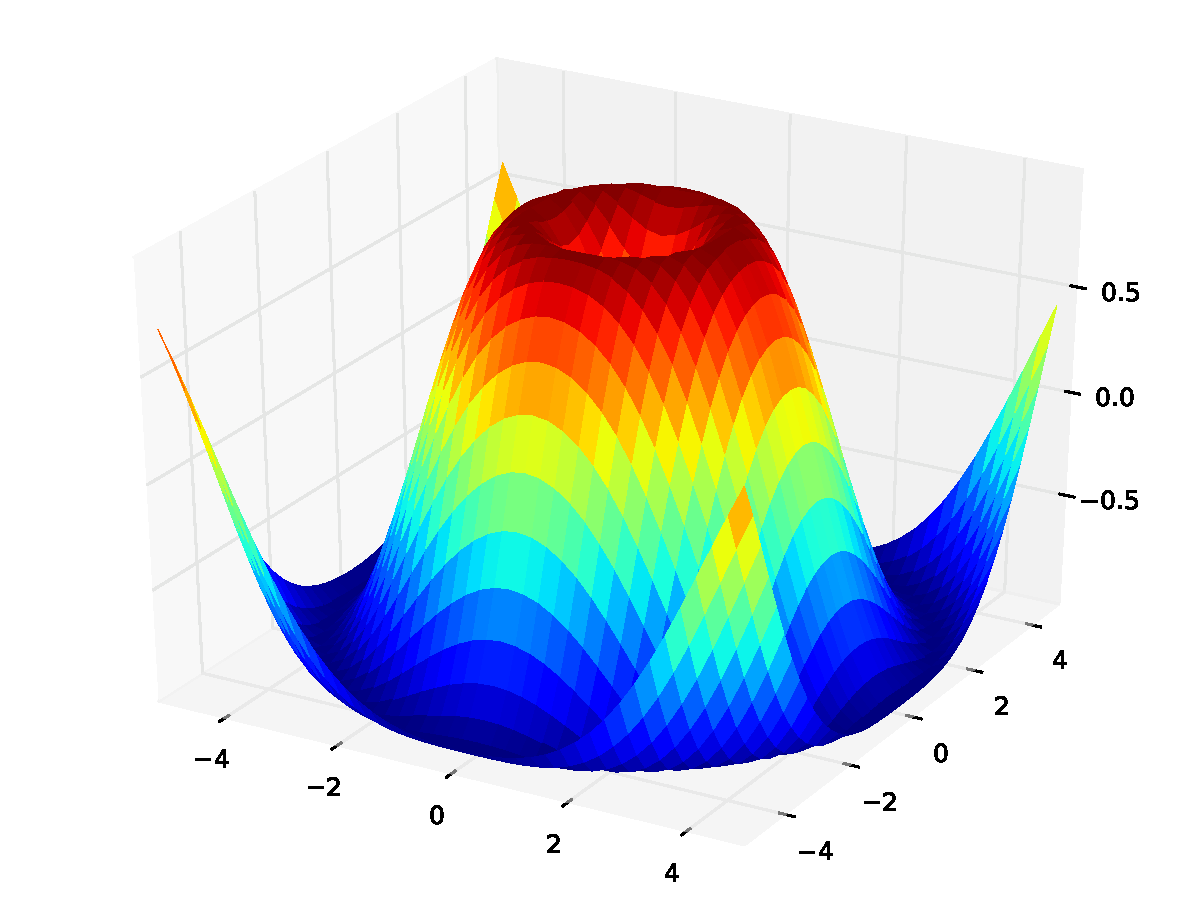
\includegraphics[width=0.6\textwidth]{Chapter-2/figs/threed}
  \caption{A figure in the appendix.}
  \label{fig:app}
\end{figure}
%
\lipsum[7-10]
\begin{table}
  \caption{A table in the appendix.}
  \label{tab:app}
  \begin{center}
    \begin{tabular}{lc}
      \toprule
      System & Author \\
      \midrule
      \TeX   & Donald Knuth   \\
      \LaTeX & Leslie Lamport \\
      \bottomrule
    \end{tabular}
  \end{center}
\end{table}
%

\section{A Second Section}

\lipsum[14-15]


\restoregeometry

%%---------------------------------------------------------------------------%%
%\ensureoddstart
\backmatter


\end{document}